\documentclass{beamer}

\mode<presentation> {
\usetheme{Madrid}
}

\usepackage{graphicx}
\usepackage{booktabs}
\usepackage{bm}
\usepackage[export]{adjustbox}
\graphicspath{{../images/}}
\usepackage{amsmath}

%------------------------------------------------

\title[LSMA]{Linear Spectral Mixture Analysis (LSMA)}

\author{Bernard Lampe}
\date{November 14, 2018}

\begin{document}
%------------------------------------------------
\begin{frame}
\titlepage
\end{frame}

%------------------------------------------------
\begin{frame}{Overview}
\tableofcontents
\end{frame}

%------------------------------------------------
\section{Overview}
\subsection{Hyperspectral Data}
    \subsubsection{Target Implanted, Scenario 2}
    \subsubsection{Target Embedded, Scenario 2}
\subsection{Fully Constrained Linear Spectral Mixture Analysis Results}
    \subsubsection{Active Set Method}
    \subsubsection{Geometric Method}
    \subsubsection{OSP Method}
\subsection{Modified Fully Constrained Linear Spectral Mixture Analysis}
    \subsubsection{Lagrange Multipler}
    \subsubsection{Iterative Algorithm}
\subsection{Non-negative Matrix Factorization}
    \subsubsection{Direct MNF}
    \subsubsection{Hoyer Sparsity NMF}
    \subsubsection{MVC-MNF}
\section{Conclusions}


%------------------------------------------------
\begin{frame}
\frametitle{Hyperspectral Data}
\vspace*{-0.7cm}
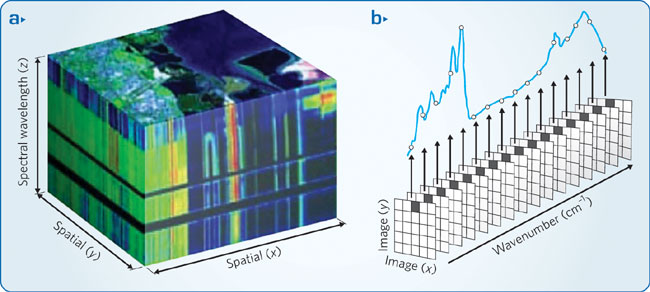
\includegraphics[width=8cm,center]{him}

[David Bannon '09]

\begin{itemize}
\item Pixels are superpositions of a finite number of materials with non-negative reflectance (ANC) and sum-to-one (ASC) constraints
\item Supervised: Applying FCLS and MFCLS to solve for abundance fractions
\item Unsupervised: Applying NMF to solve unsupervised HSI unmixing
\end{itemize}
\end{frame}

%------------------------------------------------
\begin{frame}{Synthetic Data}
\begin{columns}
    \begin{column}{0.5\textwidth}
        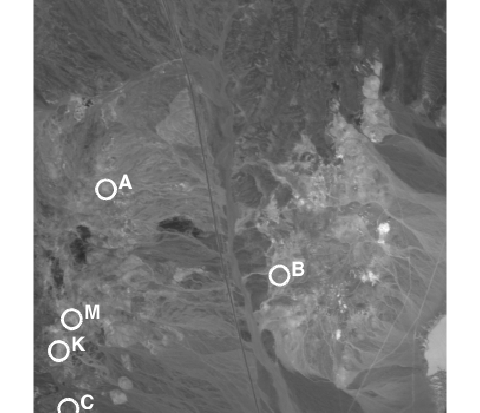
\includegraphics[width=4cm,center]{cuprite_groundTruth}
        \centering
        \\ Cuprite Dimension \(350\)x\(350\)x\(189\)

        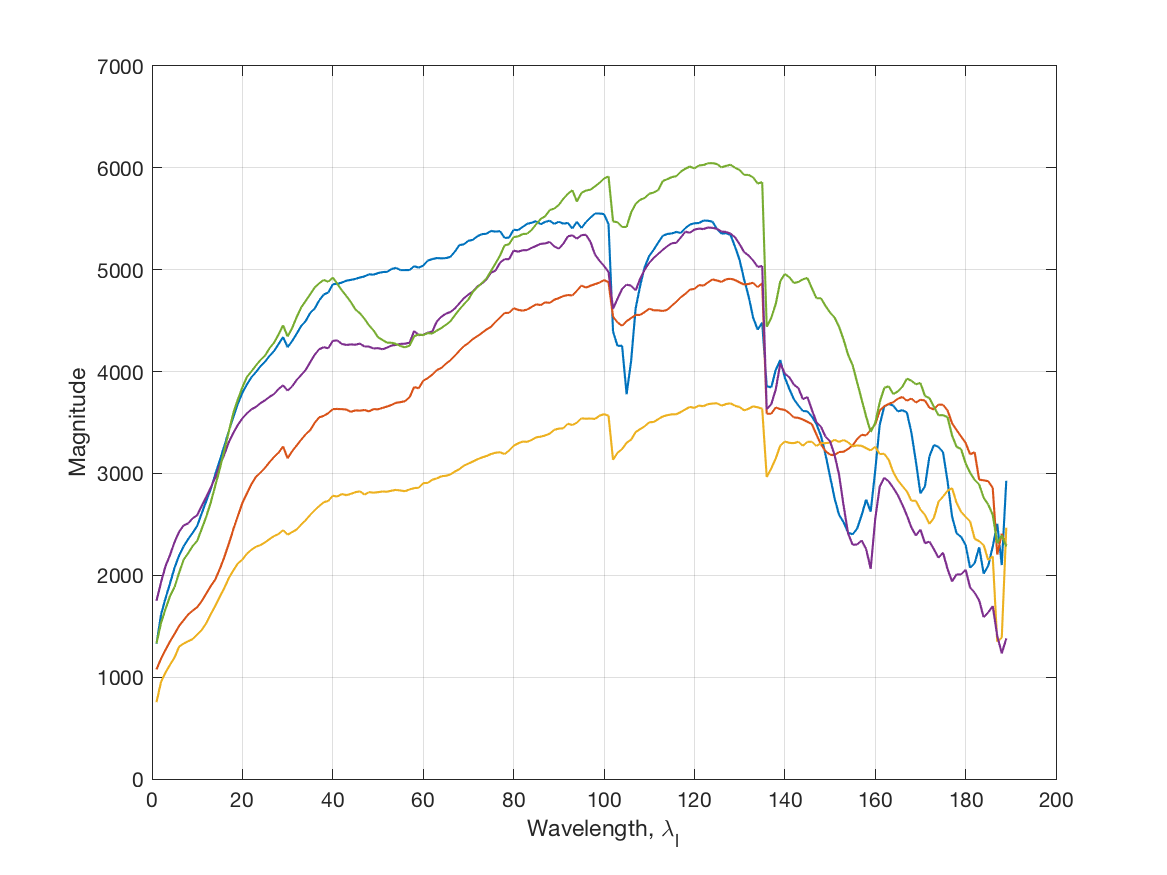
\includegraphics[width=4cm,center]{reflectance}
        \centering
        \\ Plots of marked endmembers
    \end{column}
    \begin{column}{0.5\textwidth}
        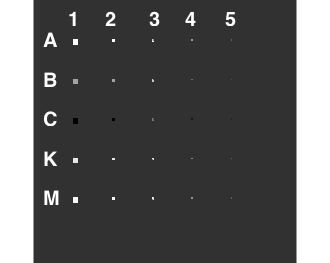
\includegraphics[width=4cm,center]{synthetic_labeled}
        \centering
        \\ Synthetic \(200\)x\(200\)x\(189\)

    \end{column}
\end{columns}
\end{frame}

%------------------------------------------------
\begin{frame}{Synthetic Data Descriptions}
        \begin{itemize}
        \item TI2 = Target Implanted, no background, SNR = 20db
        \item TE2 = Target Embedded, with background, SNR = 20db
        \item Column 1, 4x4 Pure Pixel
        \item Column 2, 2x2 Pure Pixel
        \item Column 3, 2x2 Mixed Pixel, 50\% \(\mathbf{m}_i\), 50\% \(\mathbf{m}_j\)
        \item Column 4, 1x1, Sub-pixel, 50\% pixel, 50\% background
        \item Column 5, 1x1, Sub-pixel, 25\% pixel, 75\% background
        \item Each row has one main material (A, B, C, K, M)
        \end{itemize}
\end{frame}

%------------------------------------------------
\begin{frame}{FCLS, Active Set Method}
\begin{itemize}
\item Perform NCLS on the augmented pixel and endmember matrix
\item Augment the pixel vector and endmember matrix to include ASC
\item Active set corresponds to negative components in \(\mathbf{\alpha}\)
\item Perform gradient descent on the active component dimensions only
\end{itemize}

\begin{align*}
\mathbf{s} = \begin{bmatrix}
\delta\mathbf{r} \\ 1
\end{bmatrix},
\mathbf{N} = \begin{bmatrix}
\delta \mathbf{M} \\ \mathbf{1}^T
\end{bmatrix}
\end{align*}
\end{frame}

%------------------------------------------------
\begin{frame}{FCLS, Active Set Method, TI2 Results}
\begin{columns}
    \begin{column}{0.33\textwidth}
        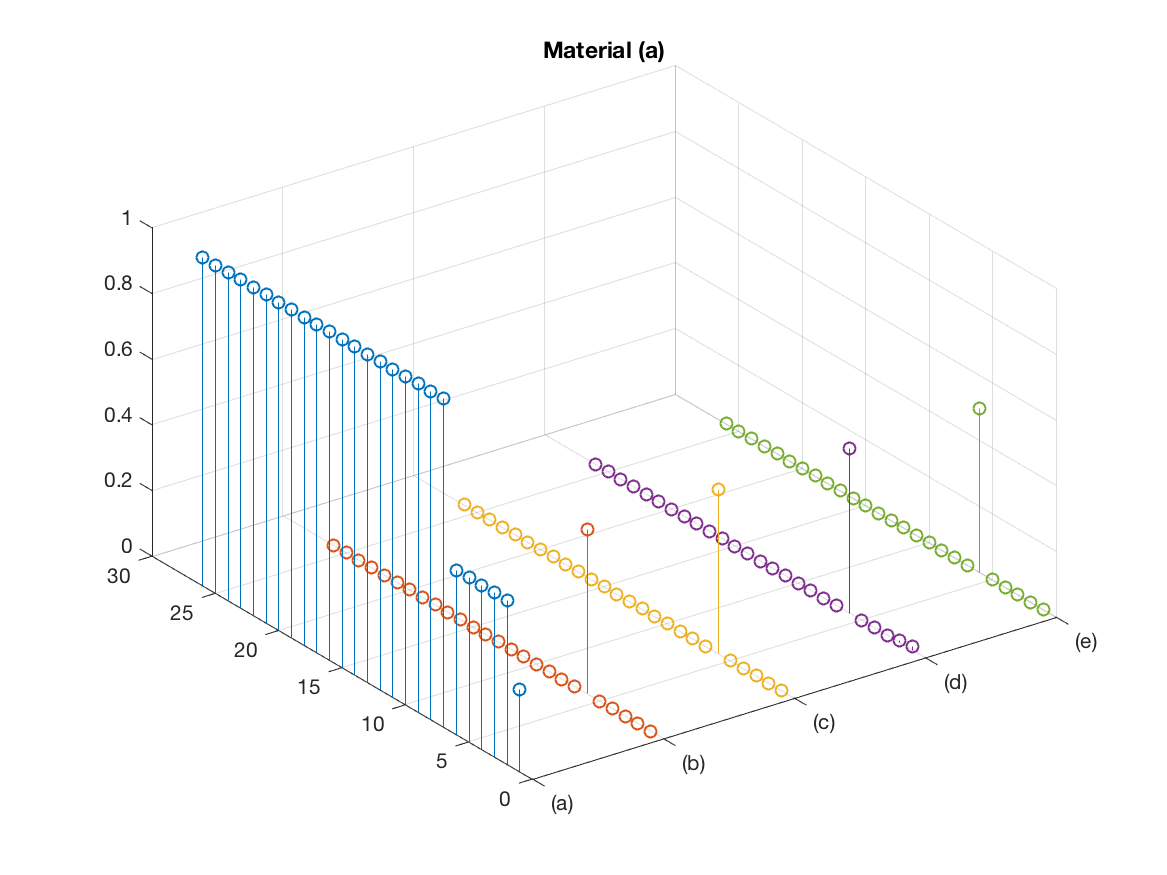
\includegraphics[width=4cm,center]{fcls_ti2_material_stem_1}
        \\ Material 1 in all rows
        \centering

        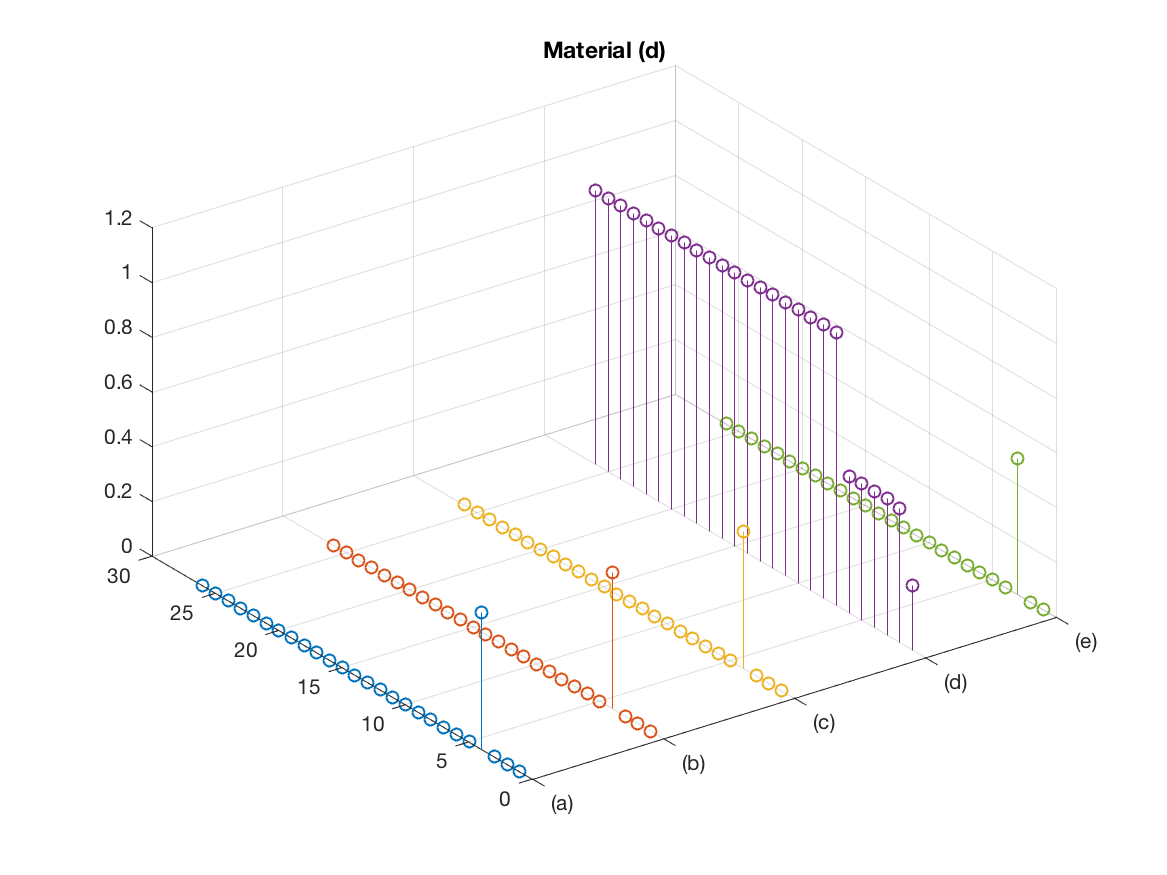
\includegraphics[width=4cm,center]{fcls_ti2_material_stem_4}
        \\ Material 4 in all rows
        \centering
    \end{column}
    \begin{column}{0.33\textwidth}
        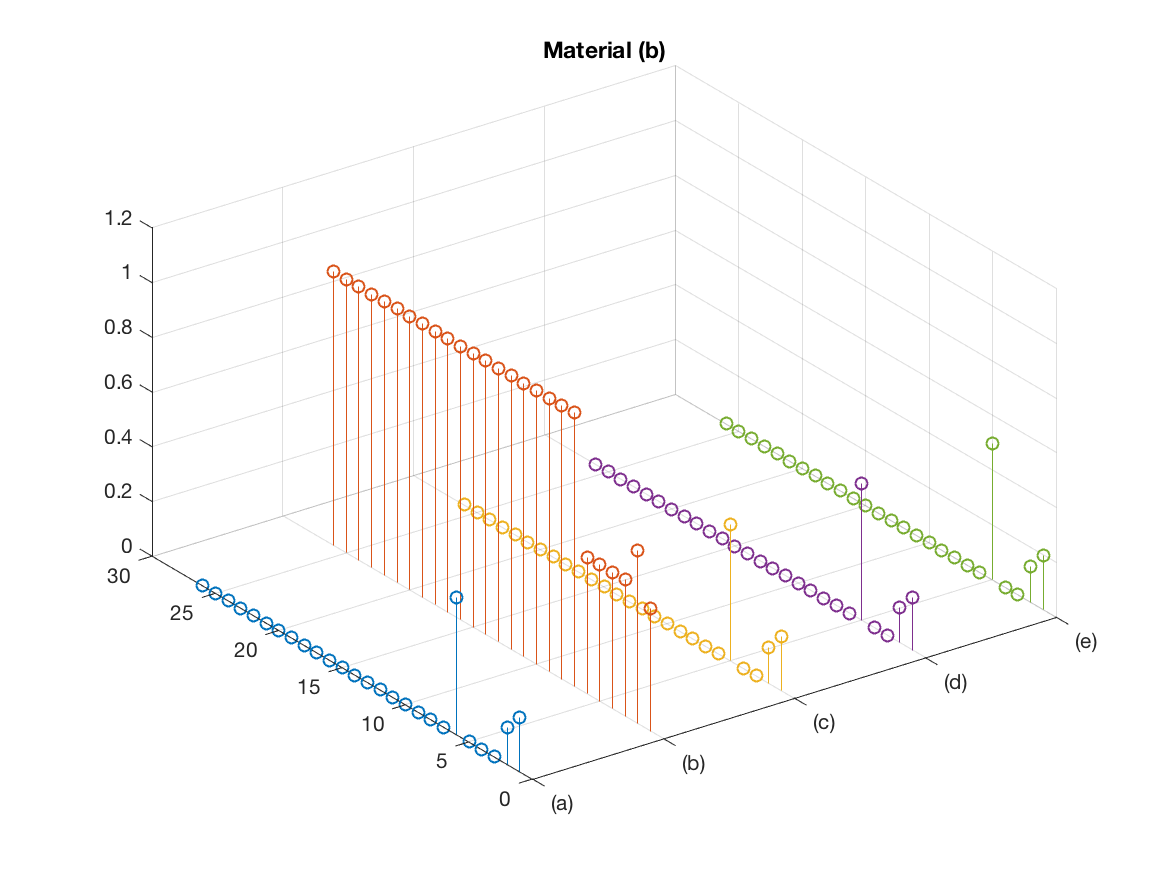
\includegraphics[width=4cm,center]{fcls_ti2_material_stem_2}
        \\ Material 2 in all rows
        \centering

        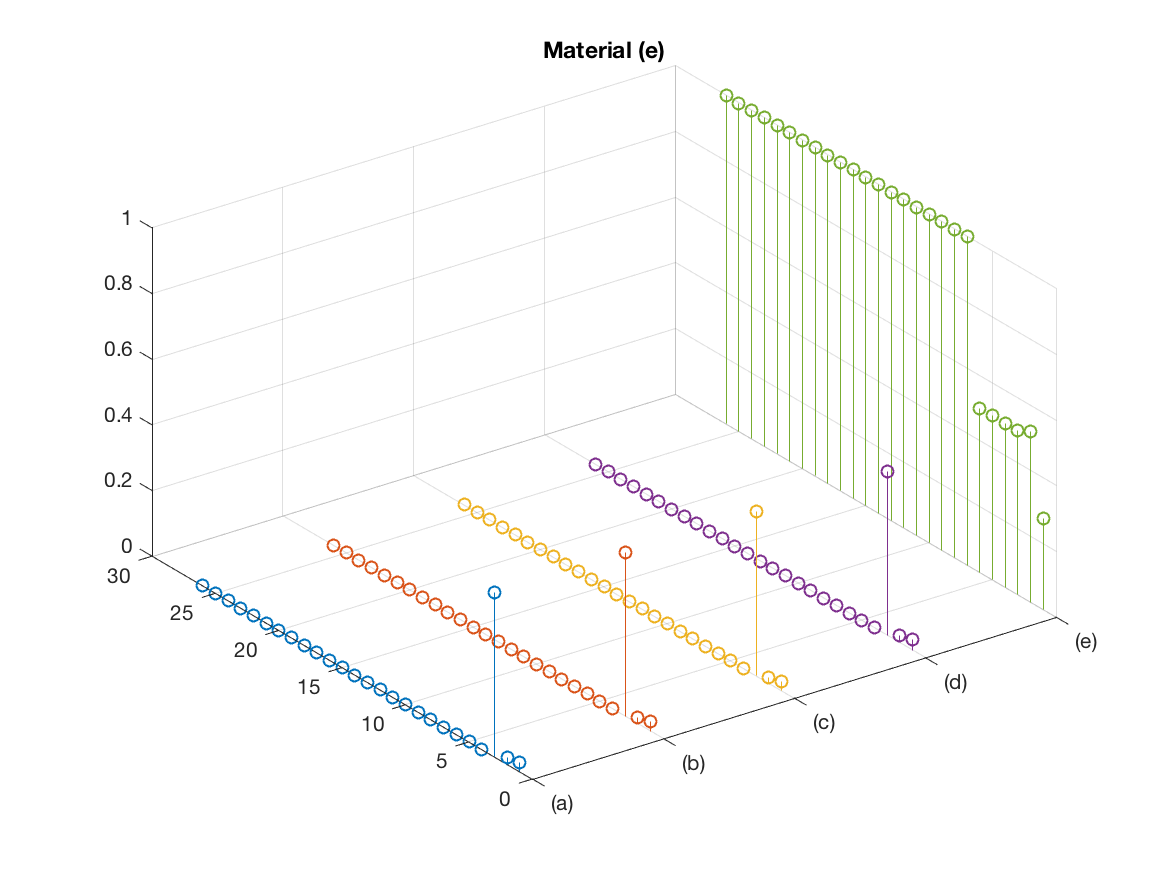
\includegraphics[width=4cm,center]{fcls_ti2_material_stem_5}
        \\ Material 5 in all rows
        \centering
    \end{column}
    \begin{column}{0.33\textwidth}
        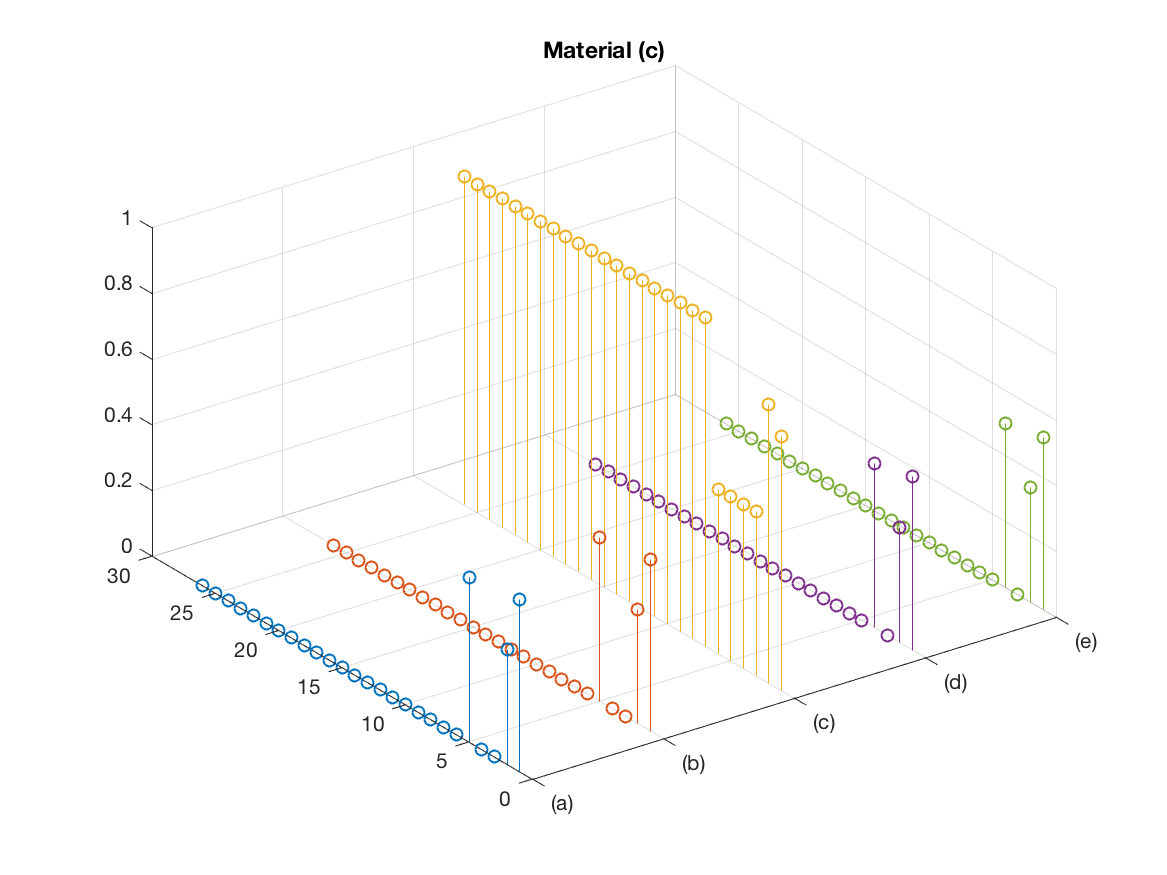
\includegraphics[width=4cm,center]{fcls_ti2_material_stem_3}
        \\ Material 3 in all rows
        \centering

        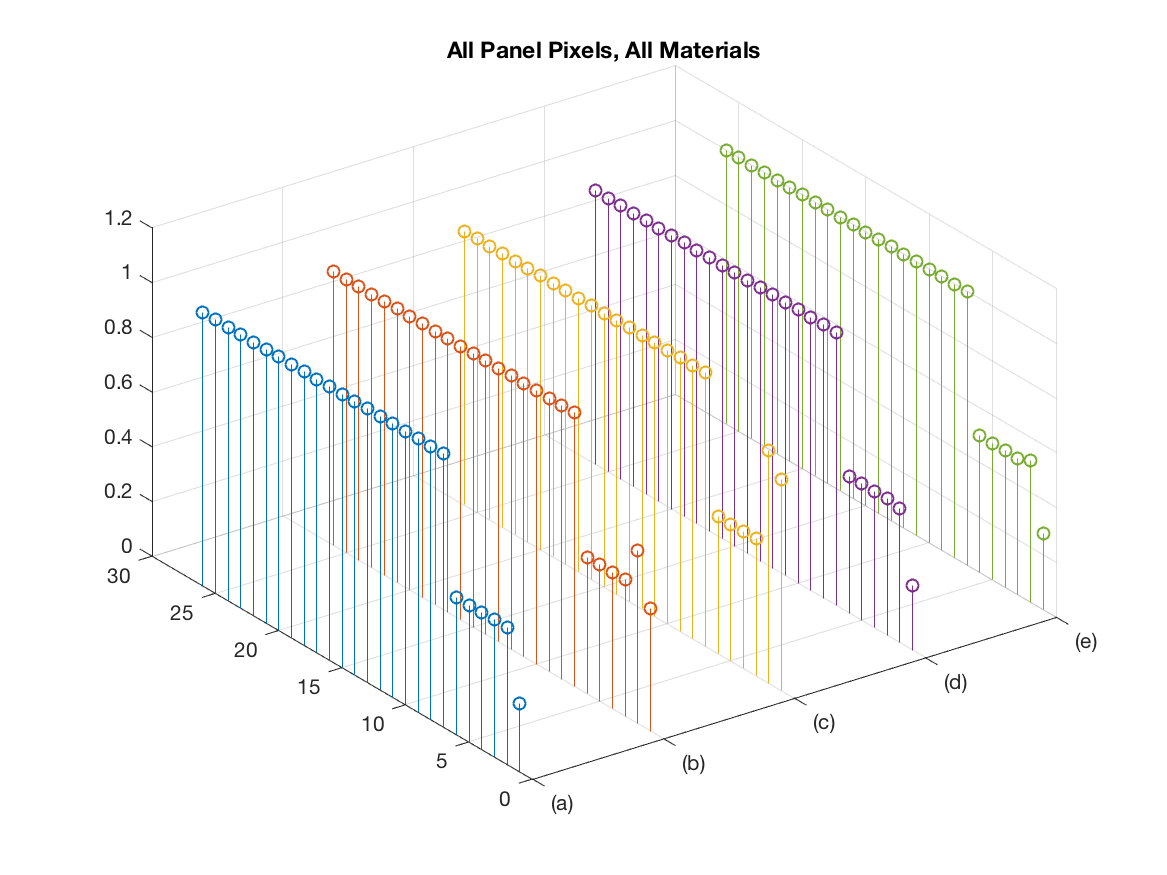
\includegraphics[width=4cm,center]{fcls_ti2_allmaterials}
        \\ All Materials
        \centering
    \end{column}
\end{columns}
\end{frame}

%------------------------------------------------
\begin{frame}{FCLS, Active Set Method, TE2 Results}
\begin{columns}
    \begin{column}{0.33\textwidth}
        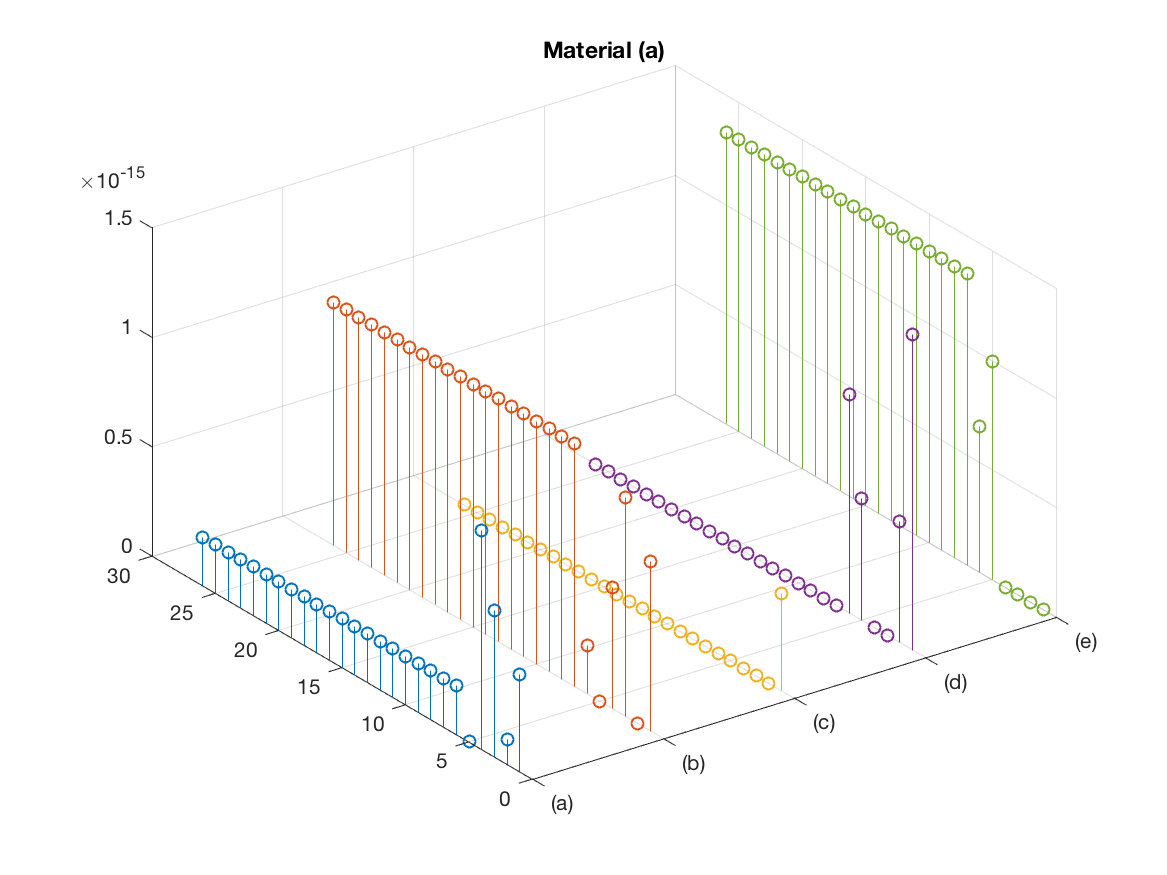
\includegraphics[width=4cm,center]{fcls_te2_material_stem_1}
        \\ Material 1 in all rows
        \centering

        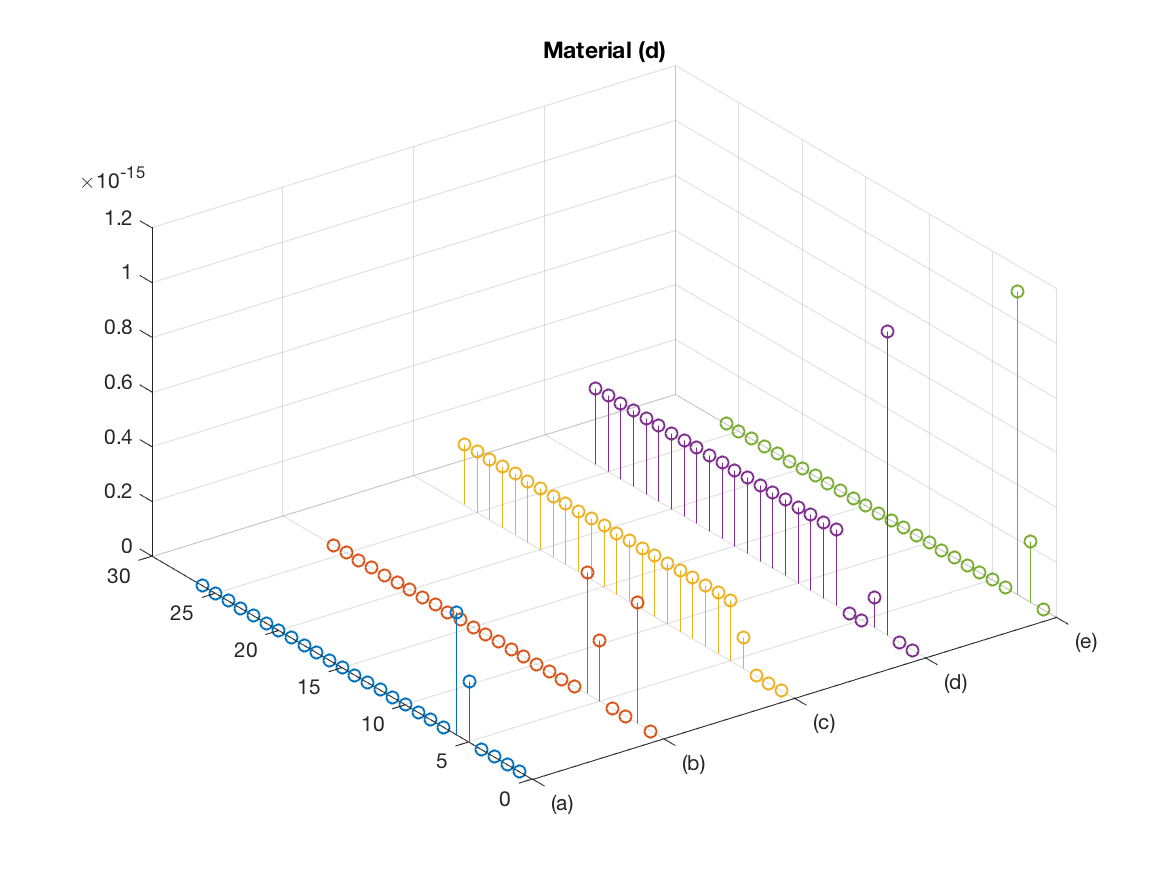
\includegraphics[width=4cm,center]{fcls_te2_material_stem_4}
        \\ Material 4 in all rows
        \centering
    \end{column}
    \begin{column}{0.33\textwidth}
        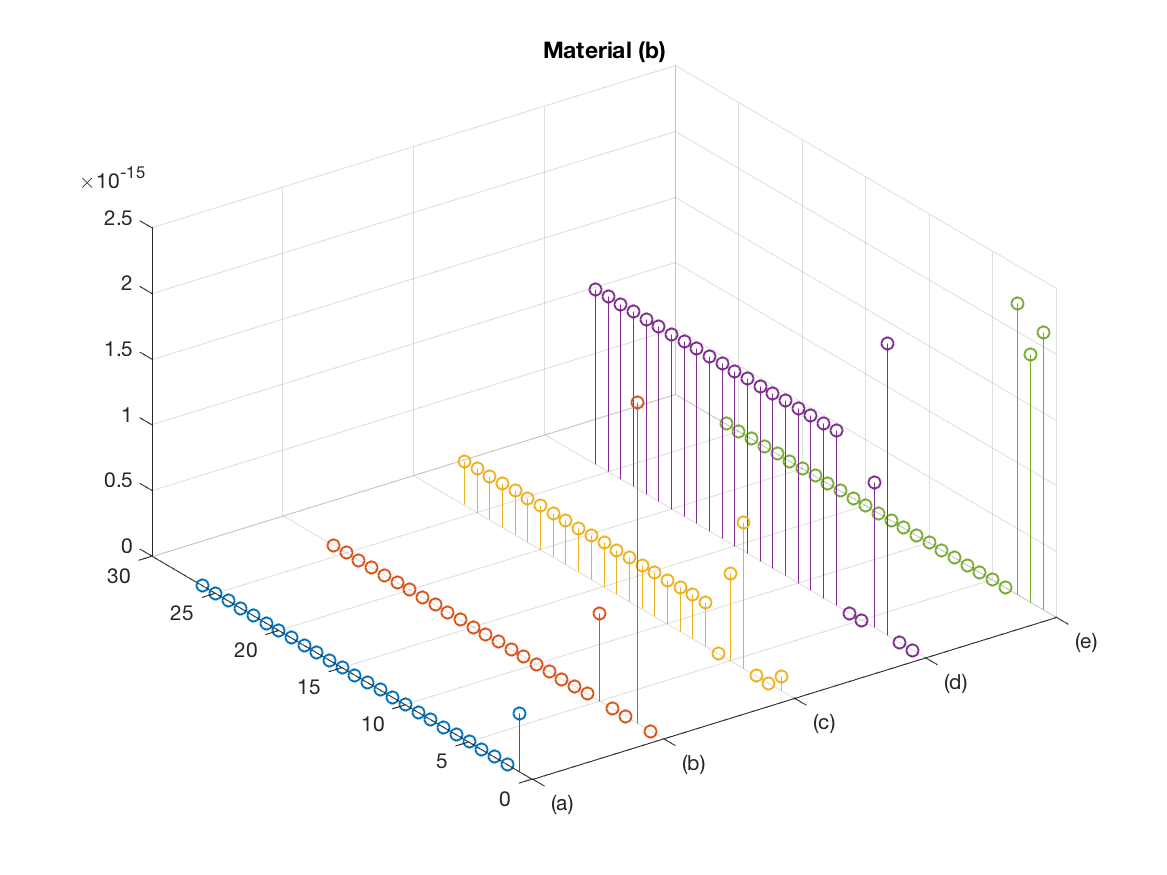
\includegraphics[width=4cm,center]{fcls_te2_material_stem_2}
        \\ Material 2 in all rows
        \centering

        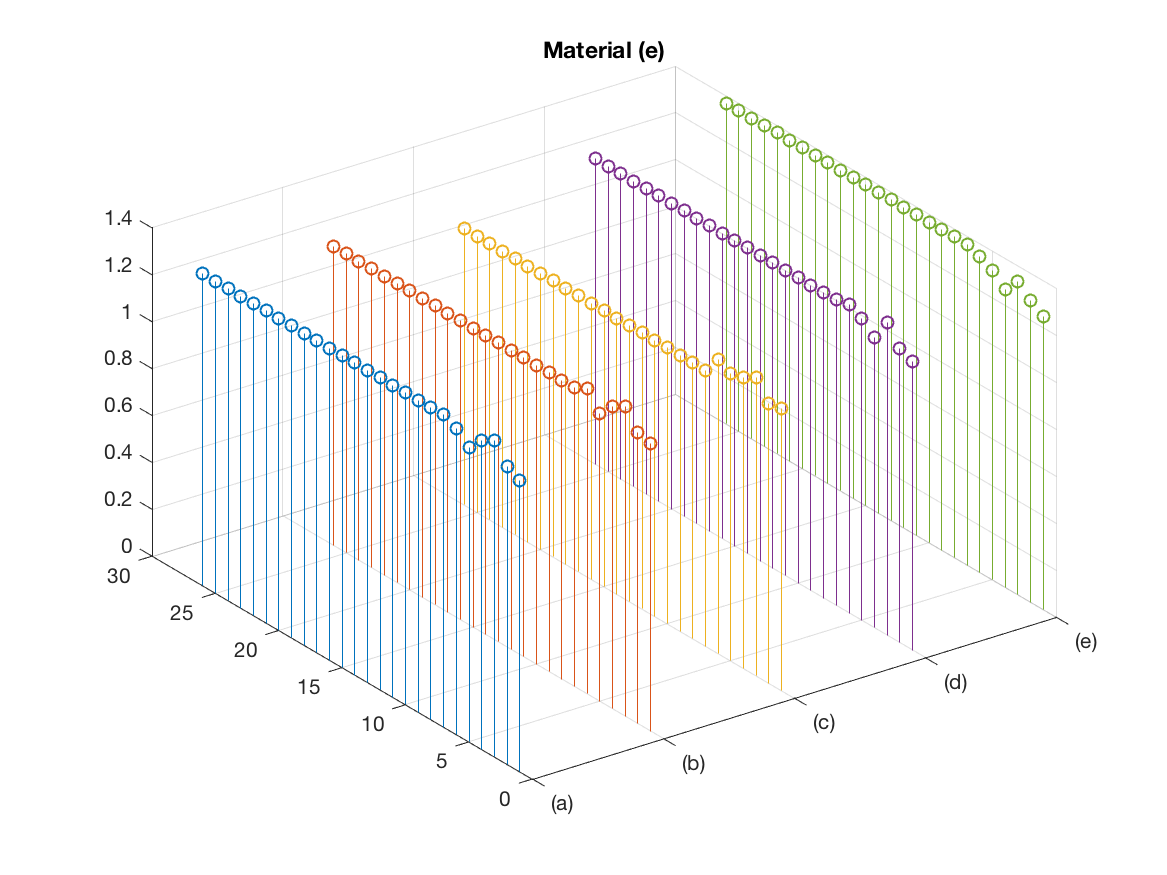
\includegraphics[width=4cm,center]{fcls_te2_material_stem_5}
        \\ Material 5 in all rows
        \centering
    \end{column}
    \begin{column}{0.33\textwidth}
        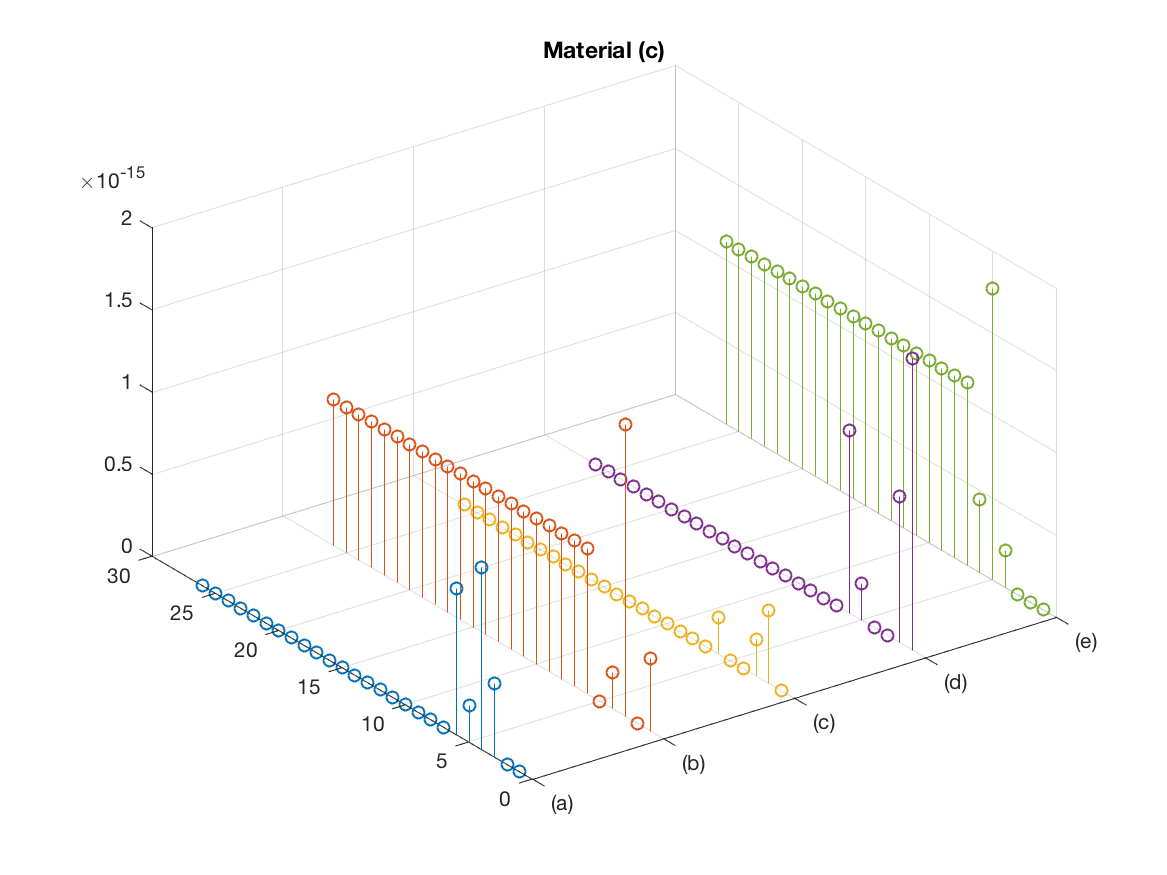
\includegraphics[width=4cm,center]{fcls_te2_material_stem_3}
        \\ Material 3 in all rows
        \centering

        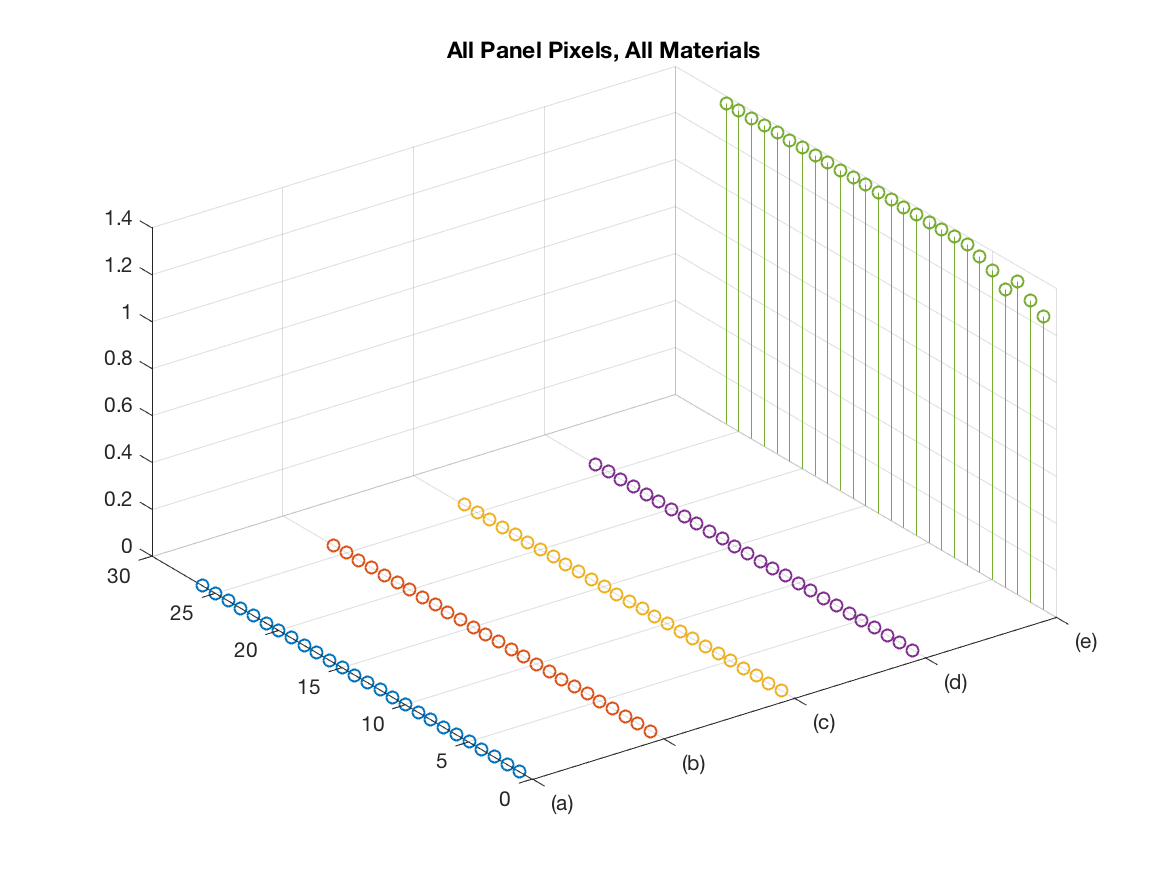
\includegraphics[width=4cm,center]{fcls_te2_allmaterials}
        \\ All Materials
        \centering
    \end{column}
\end{columns}
\end{frame}

\begin{frame}{FCLS, Geometric Method}
\begin{itemize}
\item Cramer's rule can be used to compute each component of \(\mathbf{\alpha}\).
\item The endmember matrix is augmented to add ASC.
\end{itemize}
\begin{align*}
\mathbf{\tilde{r}} = \begin{bmatrix}
1 \\ \mathbf{r}
\end{bmatrix},
\mathbf{\tilde{M}} =
\begin{bmatrix}
1 & 1 & ... & 1 \\
\mathbf{m}_1 & \mathbf{m}_2 & ... & \mathbf{m}_p
\end{bmatrix}
\end{align*}
\begin{align*}Vol(\mathbf{\tilde{m}}_1, \mathbf{\tilde{m}}_2, ..., \mathbf{\tilde{m}}_p) = \frac{1}{(p-1)!}\sqrt{|\mathbf{\tilde{M}}^T\mathbf{\tilde{M}}|}\end{align*}
\begin{align*}\alpha_i = \frac{Vol(\mathbf{\tilde{m}}_1, ..., \mathbf{\tilde{m}}_{i-1}, \mathbf{\tilde{r}}, \mathbf{\tilde{m}}_{i+1}, ..., \mathbf{\tilde{m}}_p)}{Vol(\mathbf{\tilde{m}}_1, \mathbf{\tilde{m}}_2, ..., \mathbf{\tilde{m}}_p)}\end{align*}
\end{frame}

%------------------------------------------------
\begin{frame}{FCLS, Geometric Method, TI2 Results}
\begin{columns}
    \begin{column}{0.33\textwidth}
        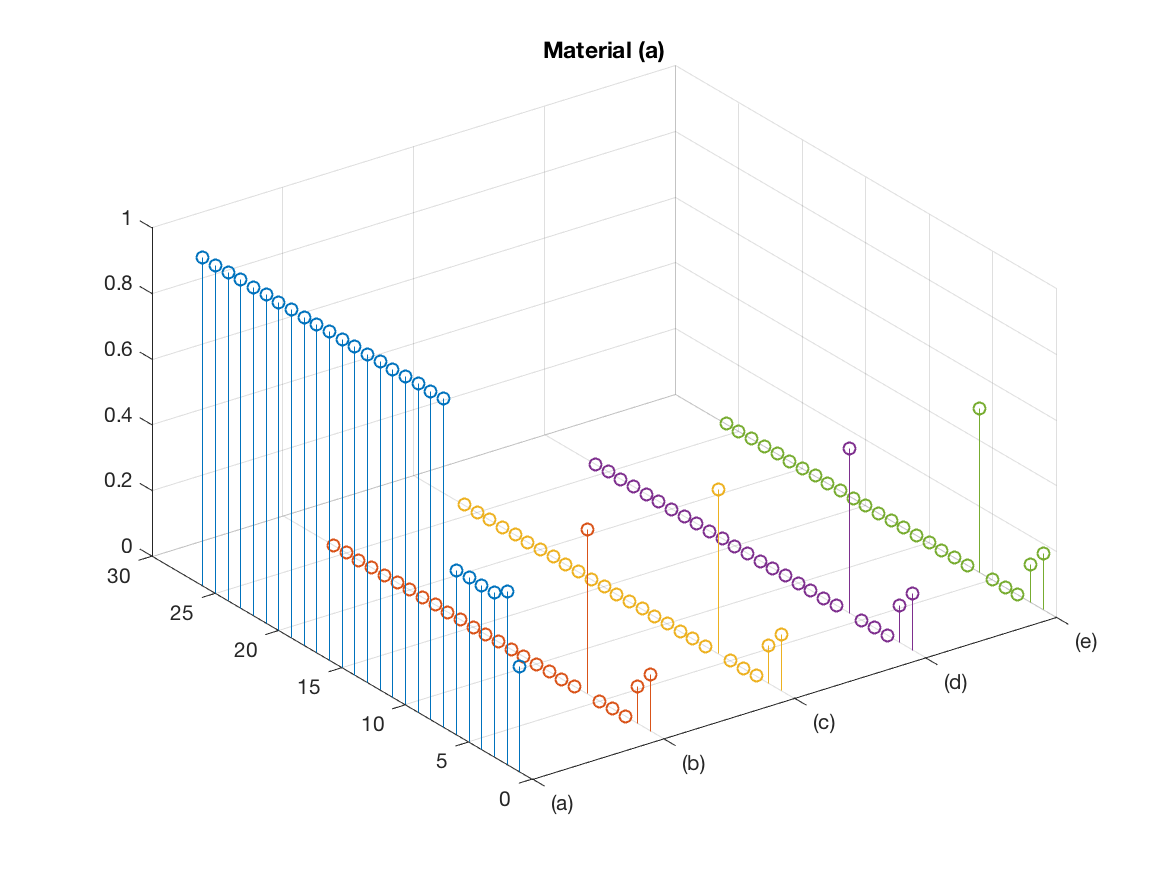
\includegraphics[width=4cm,center]{gfcls_ti2_material_stem_1}
        \\ Material 1 in all rows
        \centering

        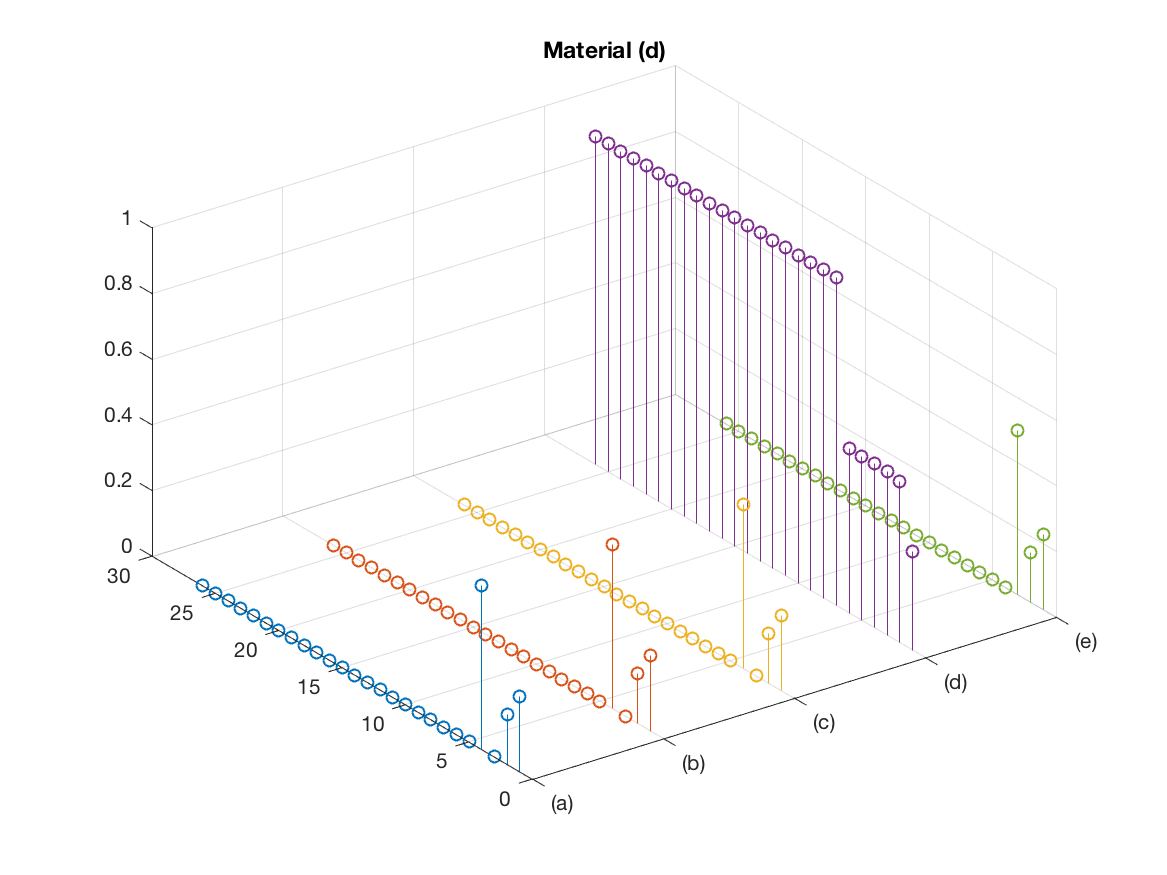
\includegraphics[width=4cm,center]{gfcls_ti2_material_stem_4}
        \\ Material 4 in all rows
        \centering
    \end{column}
    \begin{column}{0.33\textwidth}
        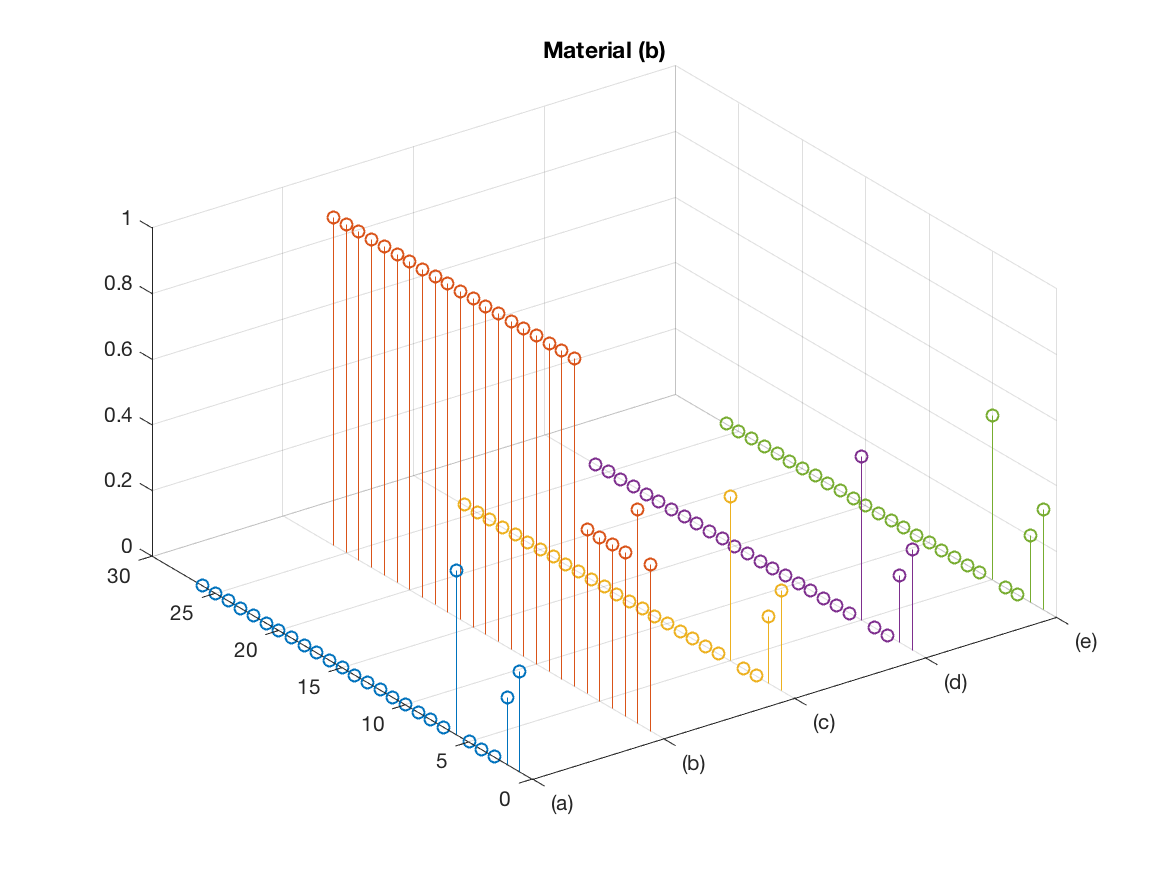
\includegraphics[width=4cm,center]{gfcls_ti2_material_stem_2}
        \\ Material 2 in all rows
        \centering

        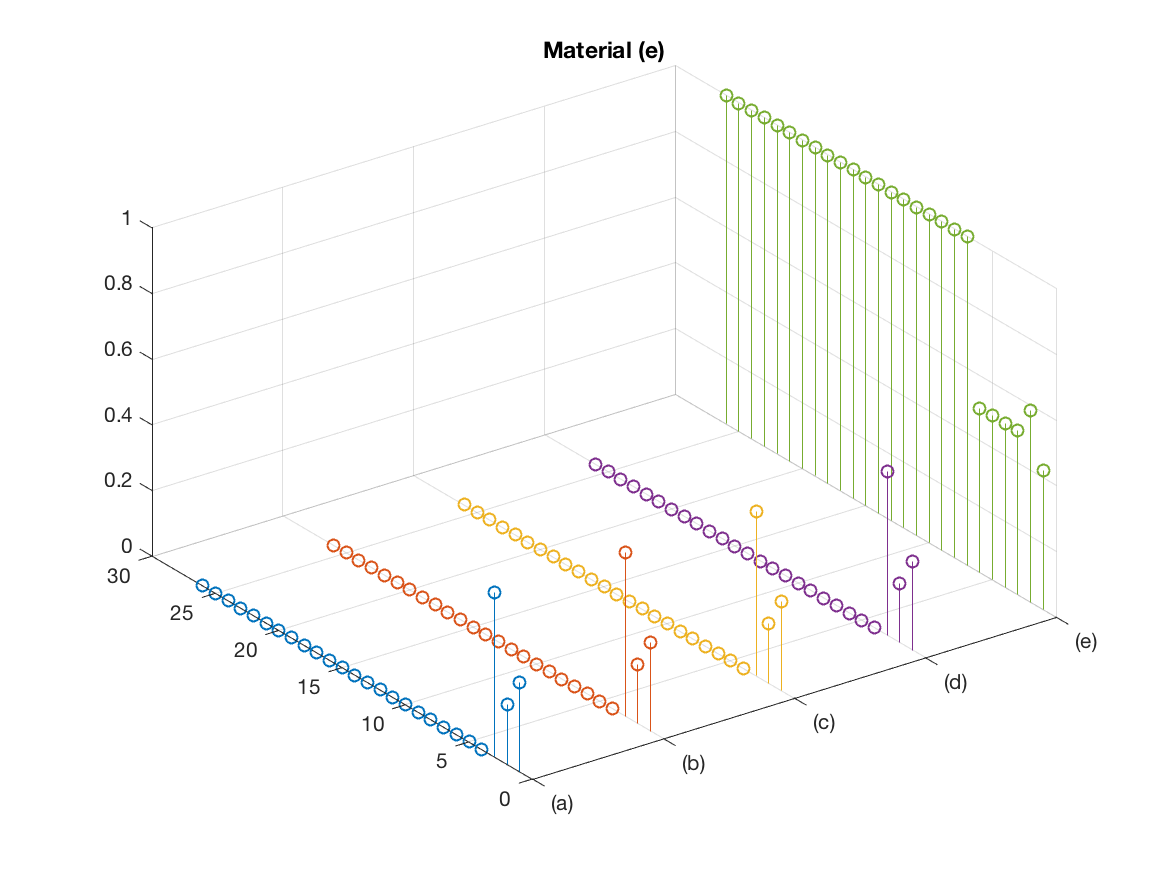
\includegraphics[width=4cm,center]{gfcls_ti2_material_stem_5}
        \\ Material 5 in all rows
        \centering
    \end{column}
    \begin{column}{0.33\textwidth}
        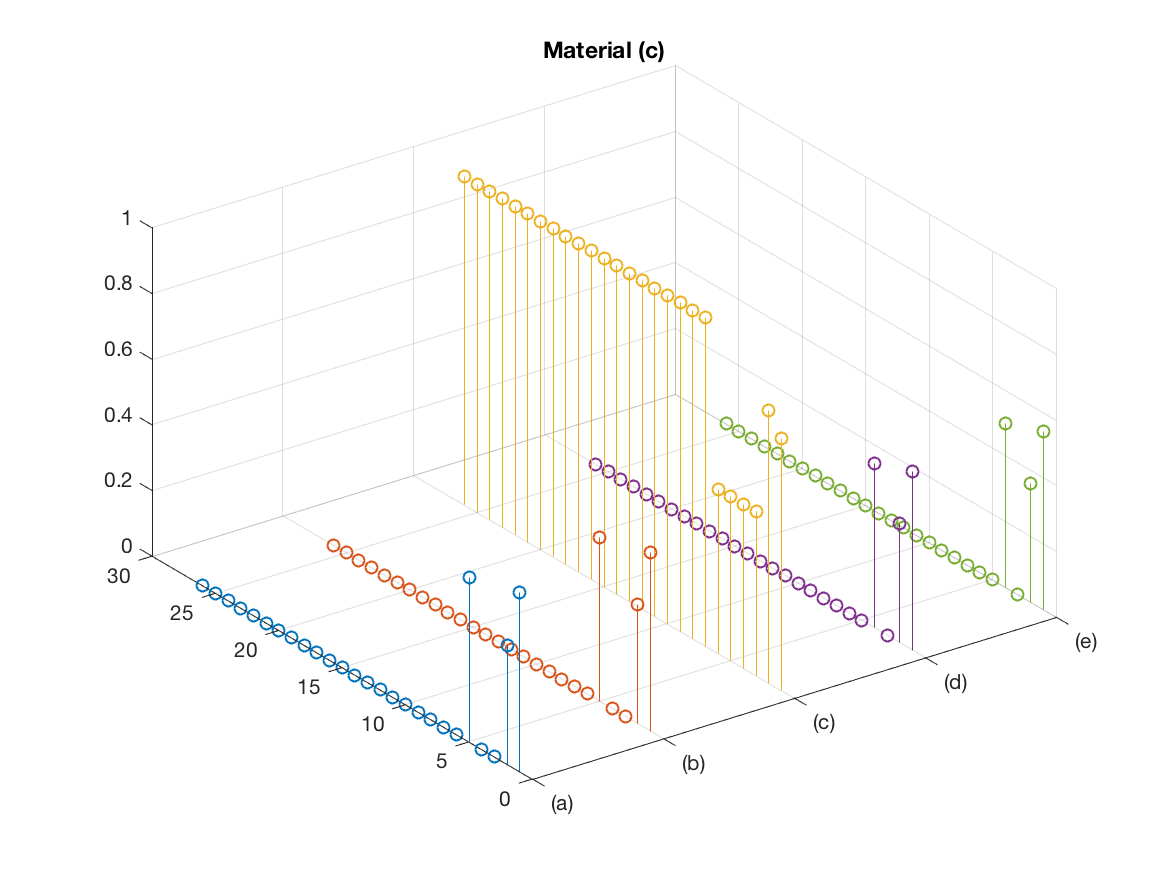
\includegraphics[width=4cm,center]{gfcls_ti2_material_stem_3}
        \\ Material 3 in all rows
        \centering

        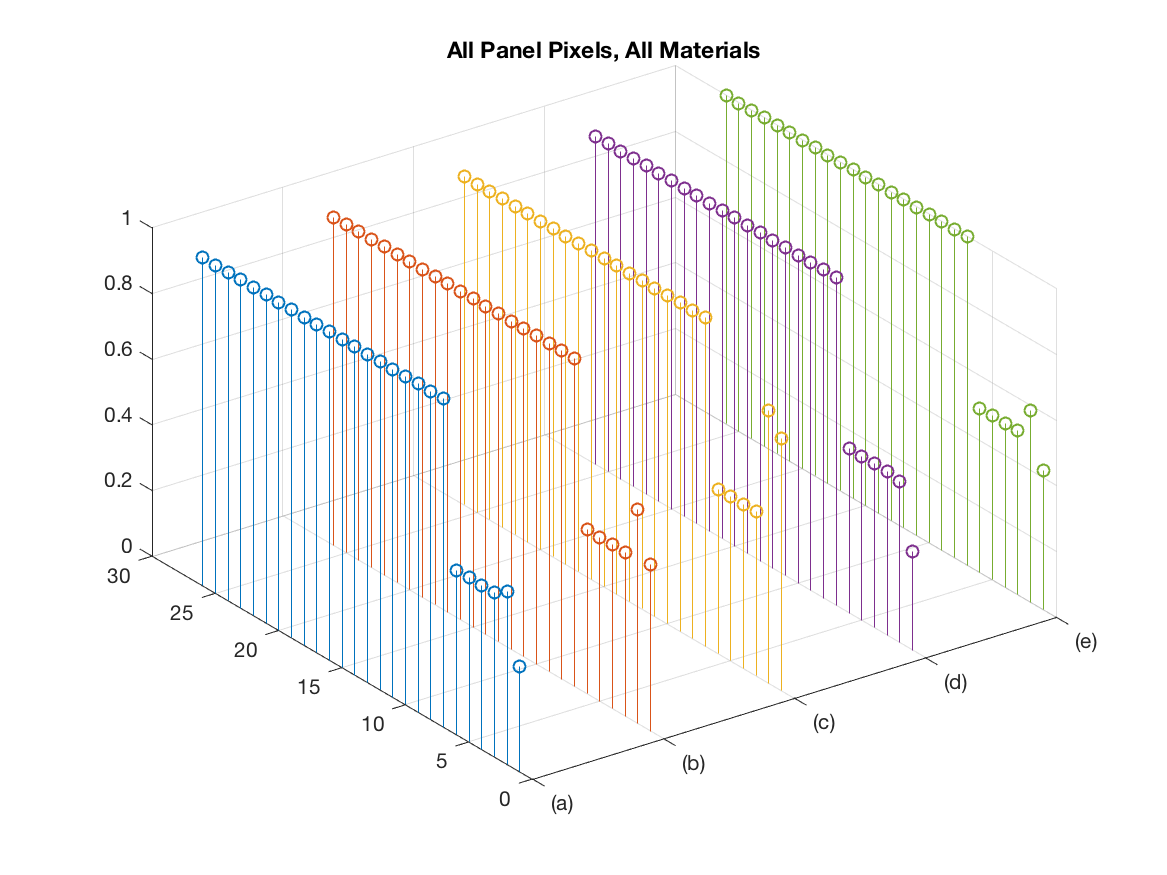
\includegraphics[width=4cm,center]{gfcls_ti2_allmaterials}
        \\ All Materials
        \centering
    \end{column}
\end{columns}
\end{frame}

%------------------------------------------------
\begin{frame}{FCLS, Geometric Method, TE2 Results}
\begin{columns}
    \begin{column}{0.33\textwidth}
        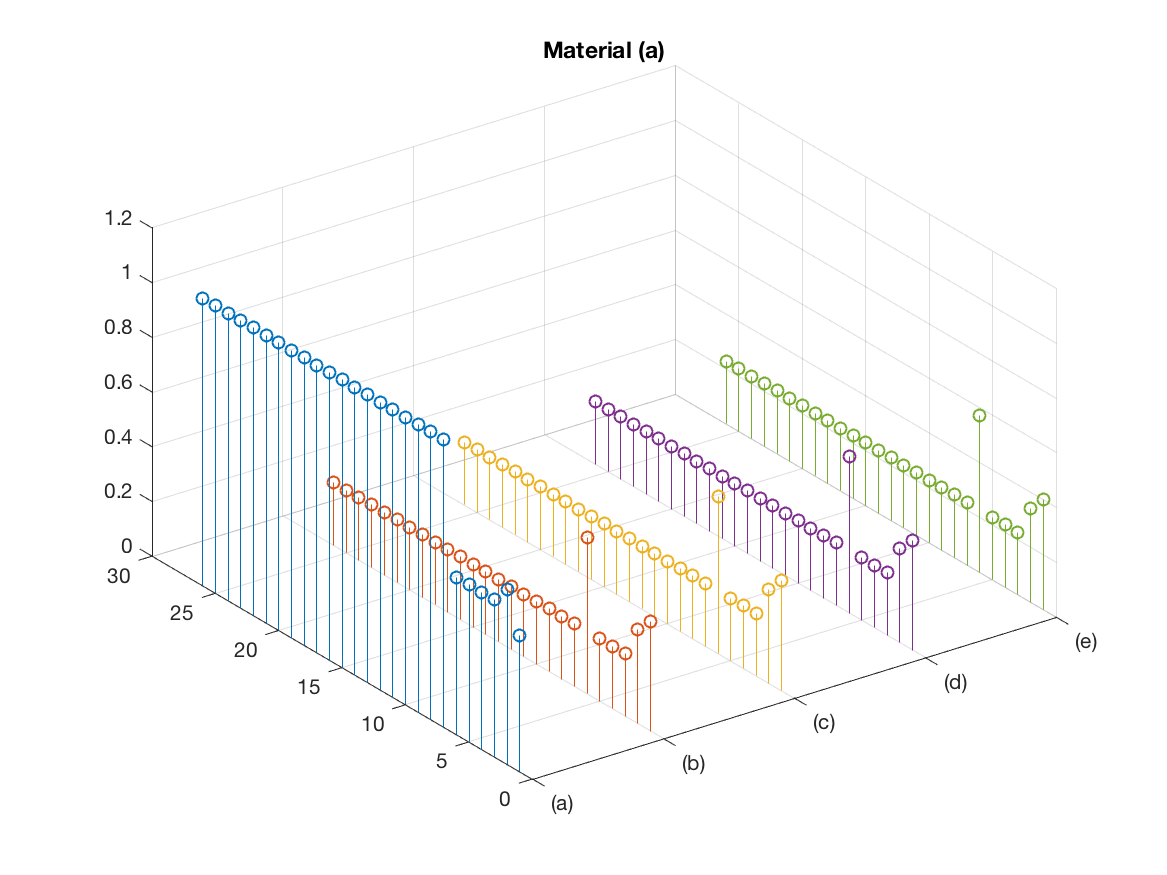
\includegraphics[width=4cm,center]{gfcls_te2_material_stem_1}
        \\ Material 1 in all rows
        \centering

        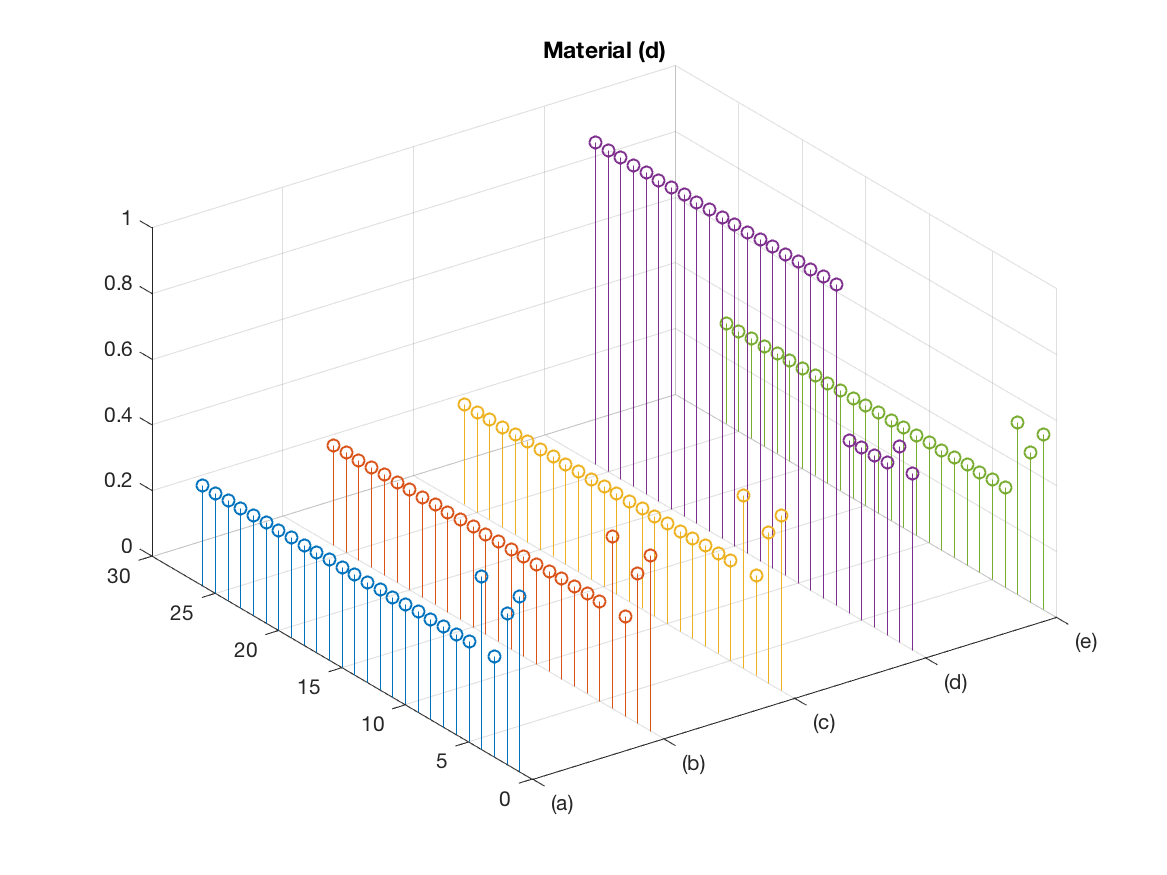
\includegraphics[width=4cm,center]{gfcls_te2_material_stem_4}
        \\ Material 4 in all rows
        \centering
    \end{column}
    \begin{column}{0.33\textwidth}
        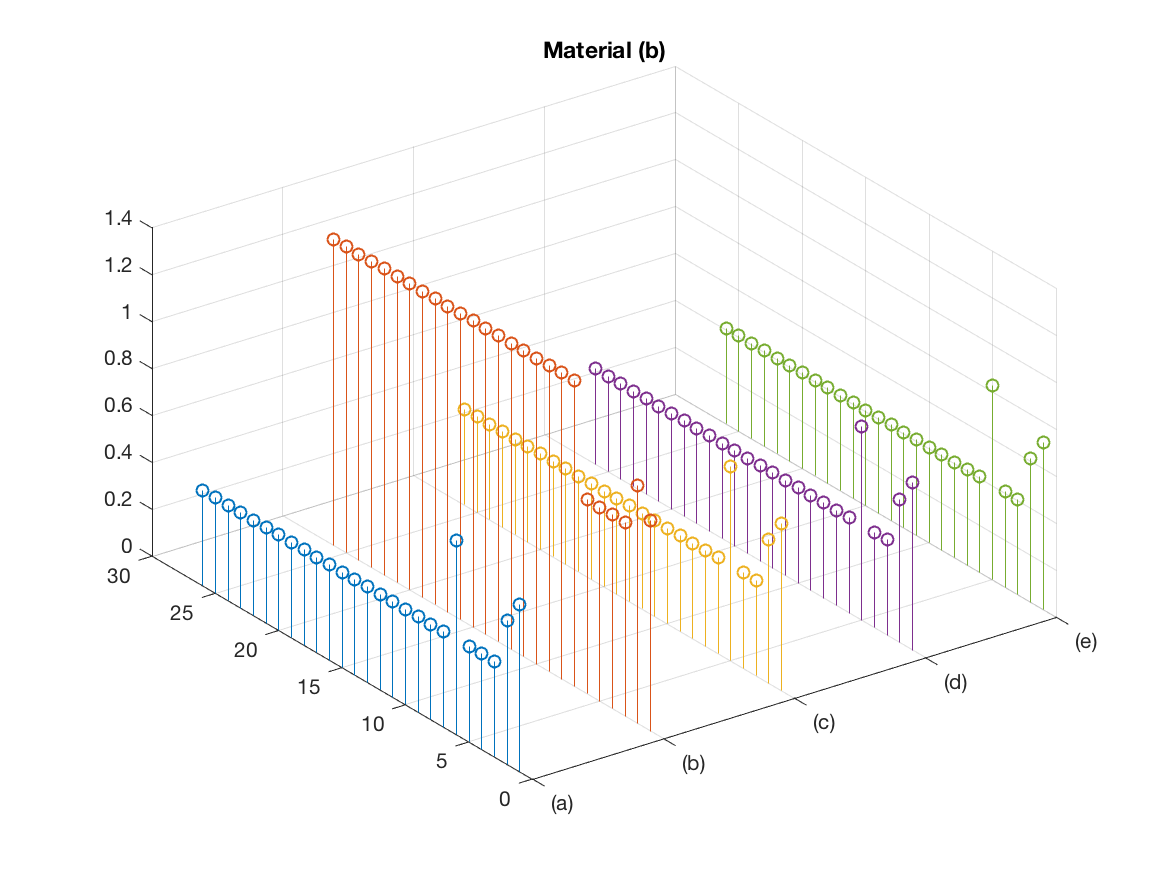
\includegraphics[width=4cm,center]{gfcls_te2_material_stem_2}
        \\ Material 2 in all rows
        \centering

        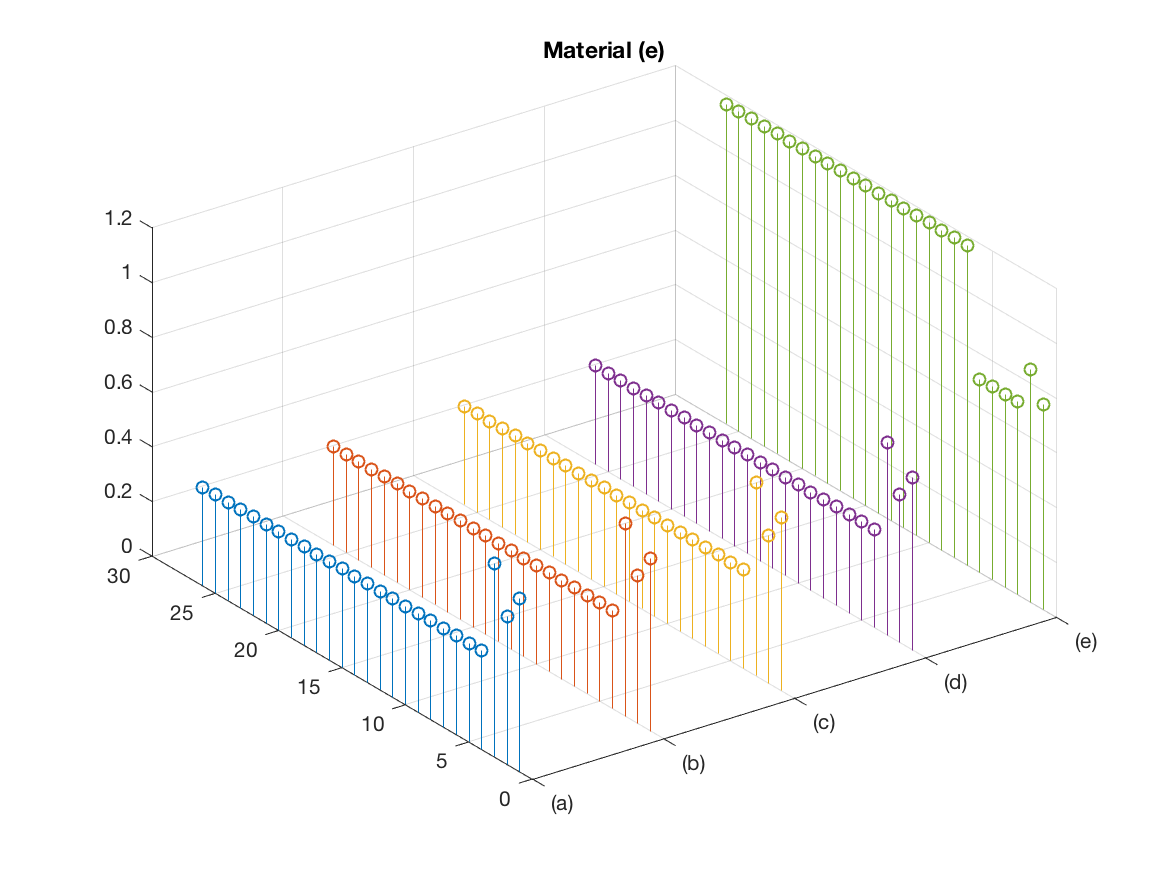
\includegraphics[width=4cm,center]{gfcls_te2_material_stem_5}
        \\ Material 5 in all rows
        \centering
    \end{column}
    \begin{column}{0.33\textwidth}
        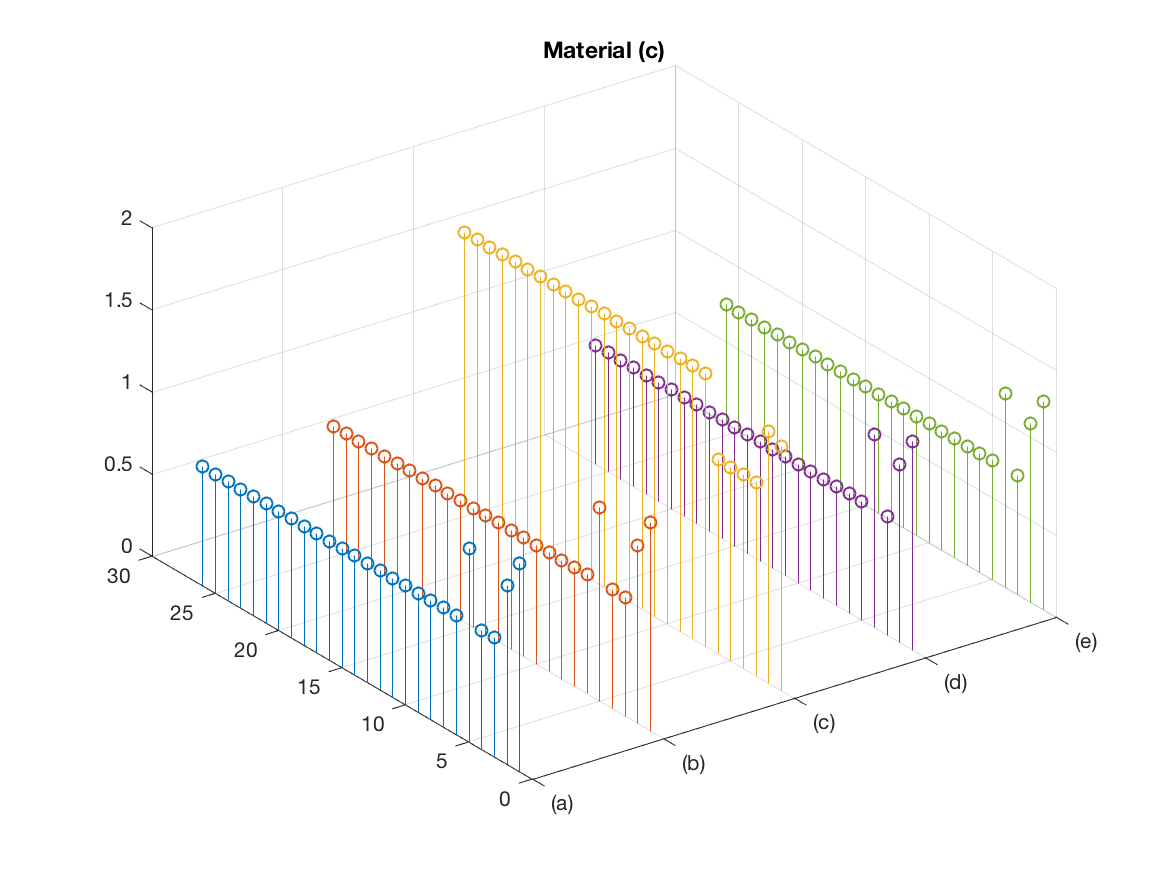
\includegraphics[width=4cm,center]{gfcls_te2_material_stem_3}
        \\ Material 3 in all rows
        \centering

        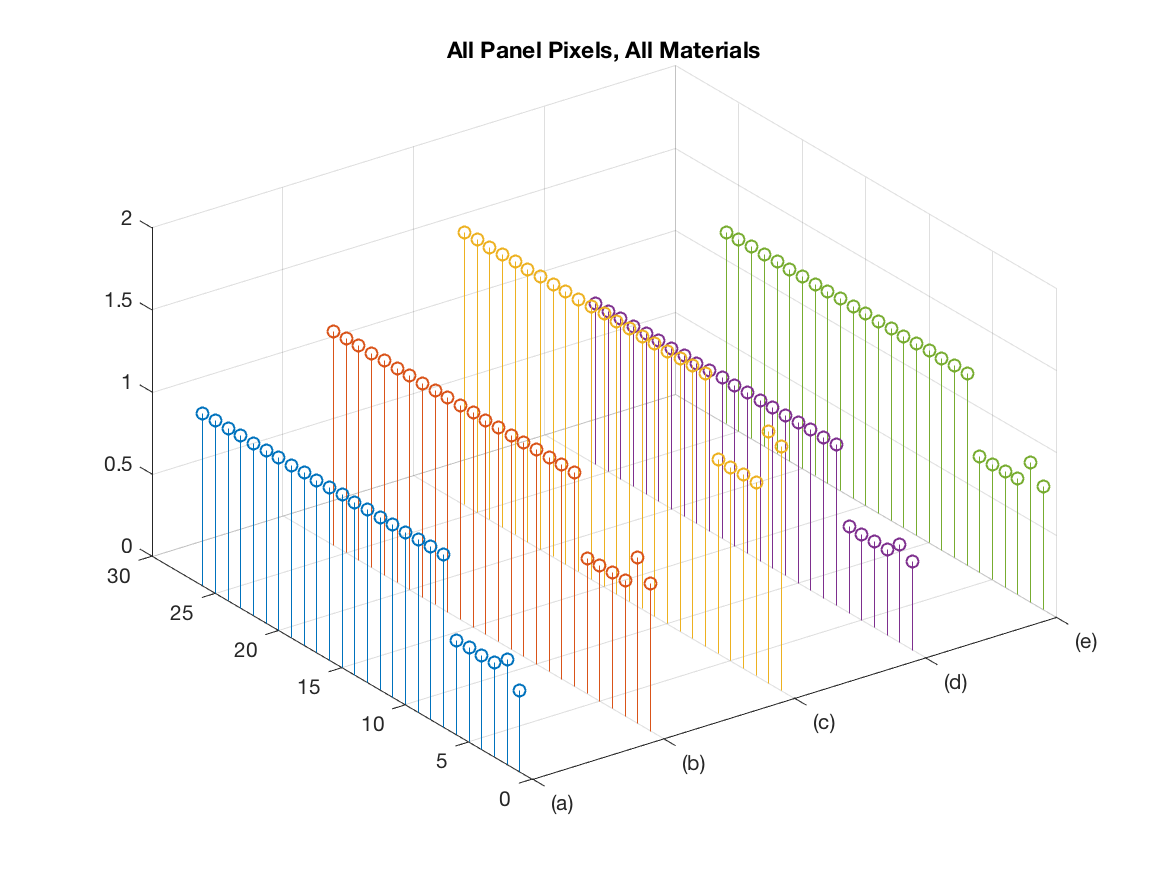
\includegraphics[width=4cm,center]{gfcls_te2_allmaterials}
        \\ All Materials
        \centering
    \end{column}
\end{columns}
\end{frame}

%------------------------------------------------
\begin{frame}{FCLS, OSP Method}
\begin{itemize}
    \item Compute \(\delta_{\mathbf{m}_i}=\mathbf{P}_{\mathbf{U}}^\perp\) classifier for all \(\mathbf{m}_i\)
    \item Classification weight is abundance fraction
    \item Suppressing background leaves endmember contribution non-negative
    \item Normalized after classification
\end{itemize}

\begin{align*}
\mathbf{\tilde{M}} = \left[\mathbf{m}_1,...,\mathbf{m}_{i-1}, \mathbf{m}_{i+1}, ..., \mathbf{m}_p\right]
\end{align*}

\begin{align*}
\delta_{\mathbf{m}_i}=\mathbf{P}_{\mathbf{U}}^\perp = \mathbf{I} - \mathbf{\tilde{M}}\left(\mathbf{\tilde{M}}^T\mathbf{\tilde{M}}\right)^{-1}\mathbf{\tilde{M}}^T
\end{align*}
\end{frame}


%------------------------------------------------
\begin{frame}{FCLS, OSP Method, TI2 Results}
\begin{columns}
    \begin{column}{0.33\textwidth}
        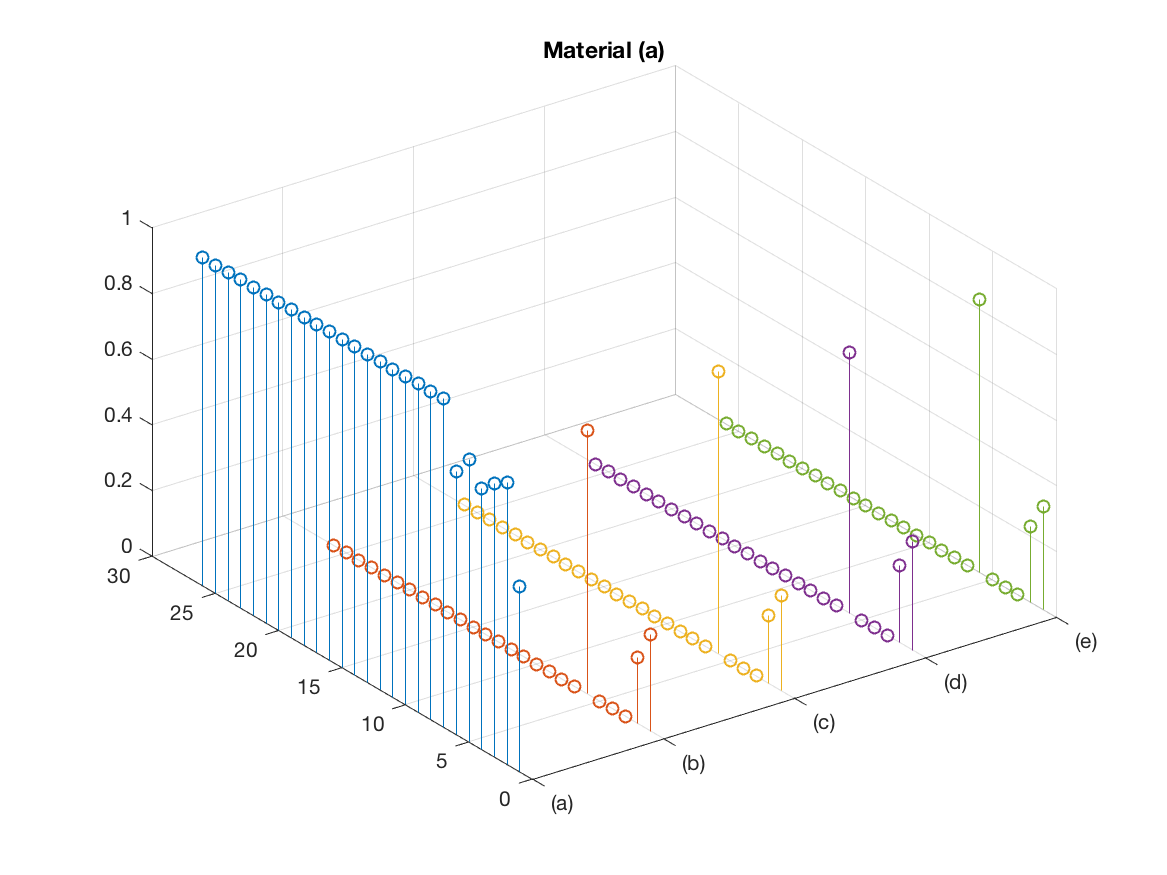
\includegraphics[width=4cm,center]{osp_fcls_ti2_material_stem_1}
        \\ Material 1 in all rows
        \centering

        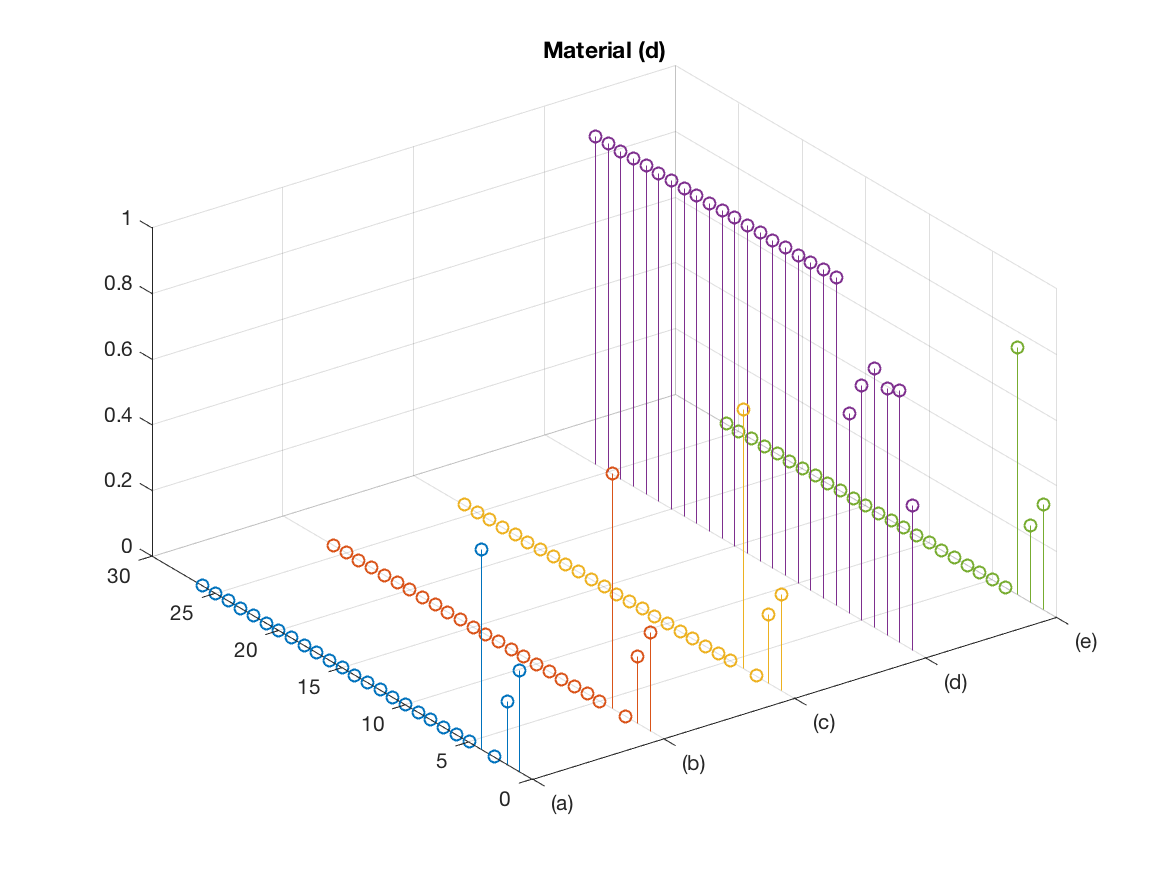
\includegraphics[width=4cm,center]{osp_fcls_ti2_material_stem_4}
        \\ Material 4 in all rows
        \centering
    \end{column}
    \begin{column}{0.33\textwidth}
        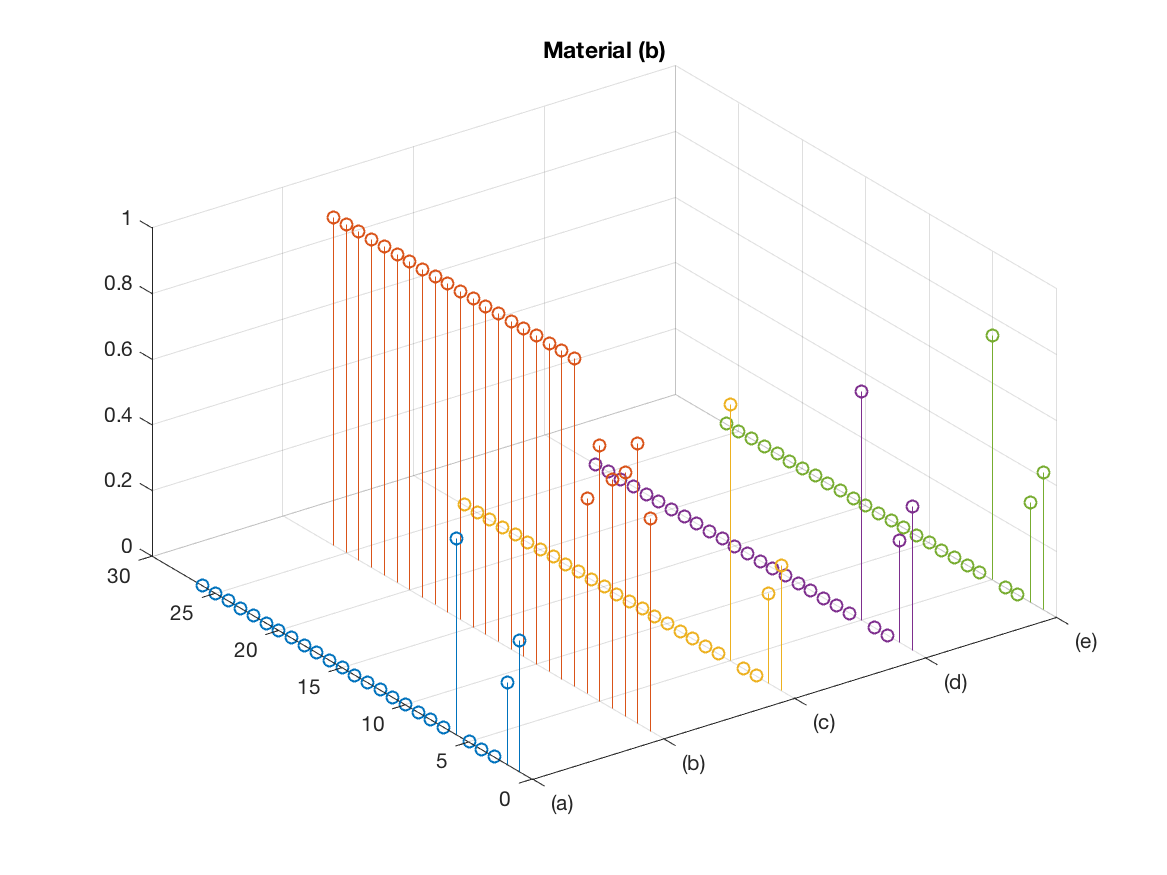
\includegraphics[width=4cm,center]{osp_fcls_ti2_material_stem_2}
        \\ Material 2 in all rows
        \centering

        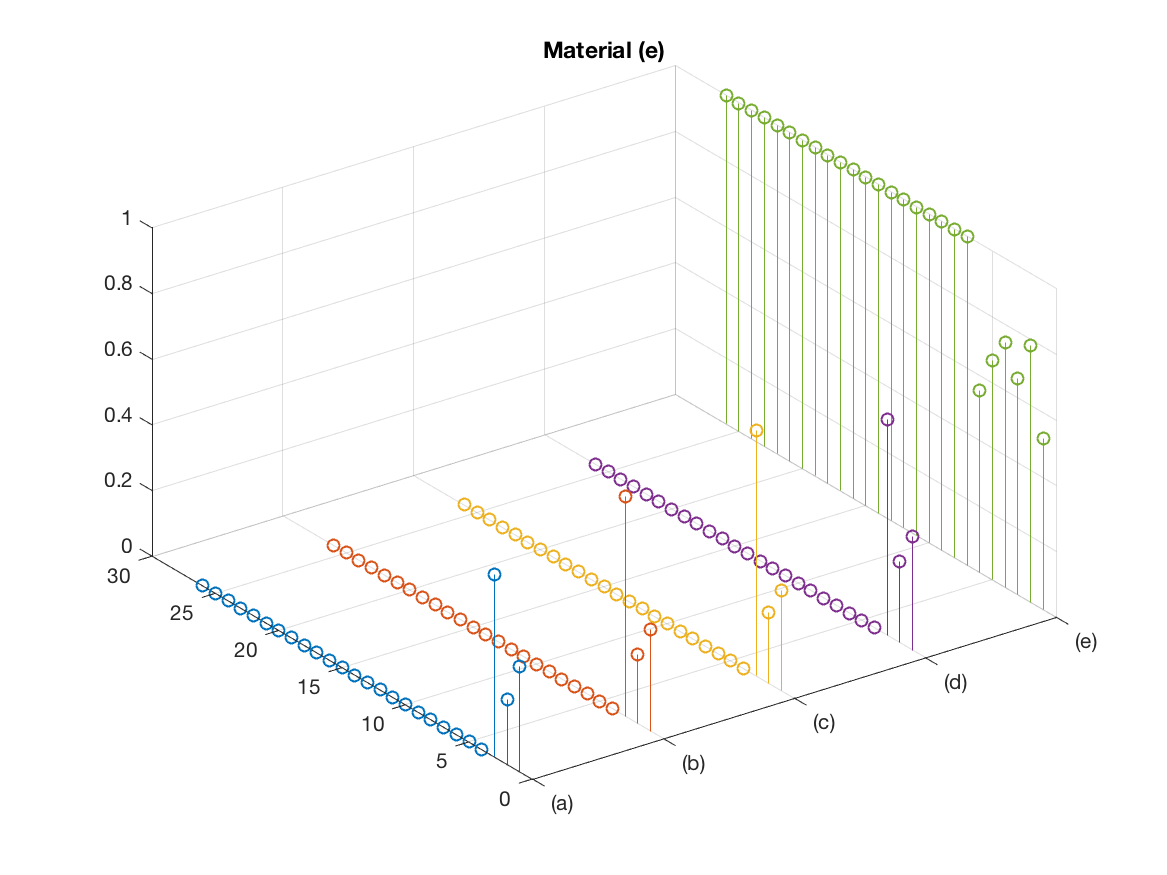
\includegraphics[width=4cm,center]{osp_fcls_ti2_material_stem_5}
        \\ Material 5 in all rows
        \centering
    \end{column}
    \begin{column}{0.33\textwidth}
        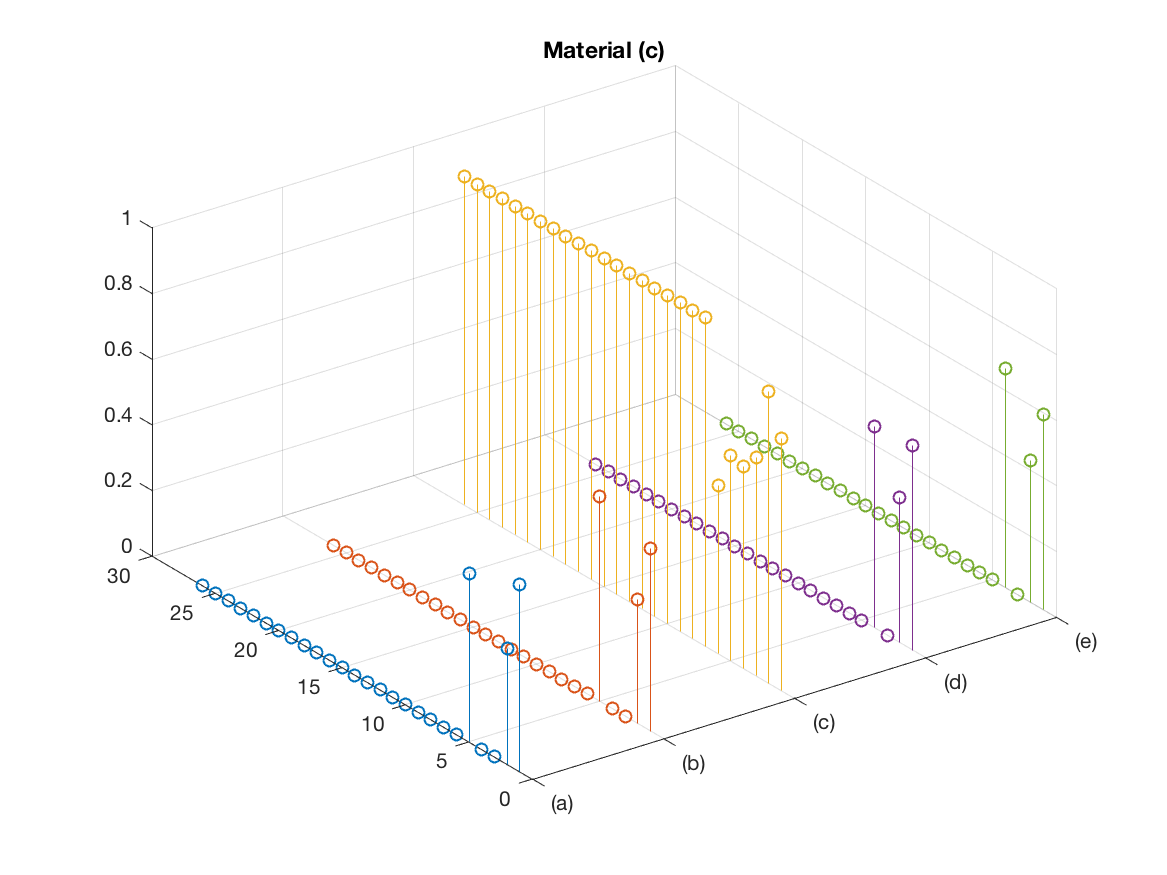
\includegraphics[width=4cm,center]{osp_fcls_ti2_material_stem_3}
        \\ Material 3 in all rows
        \centering

        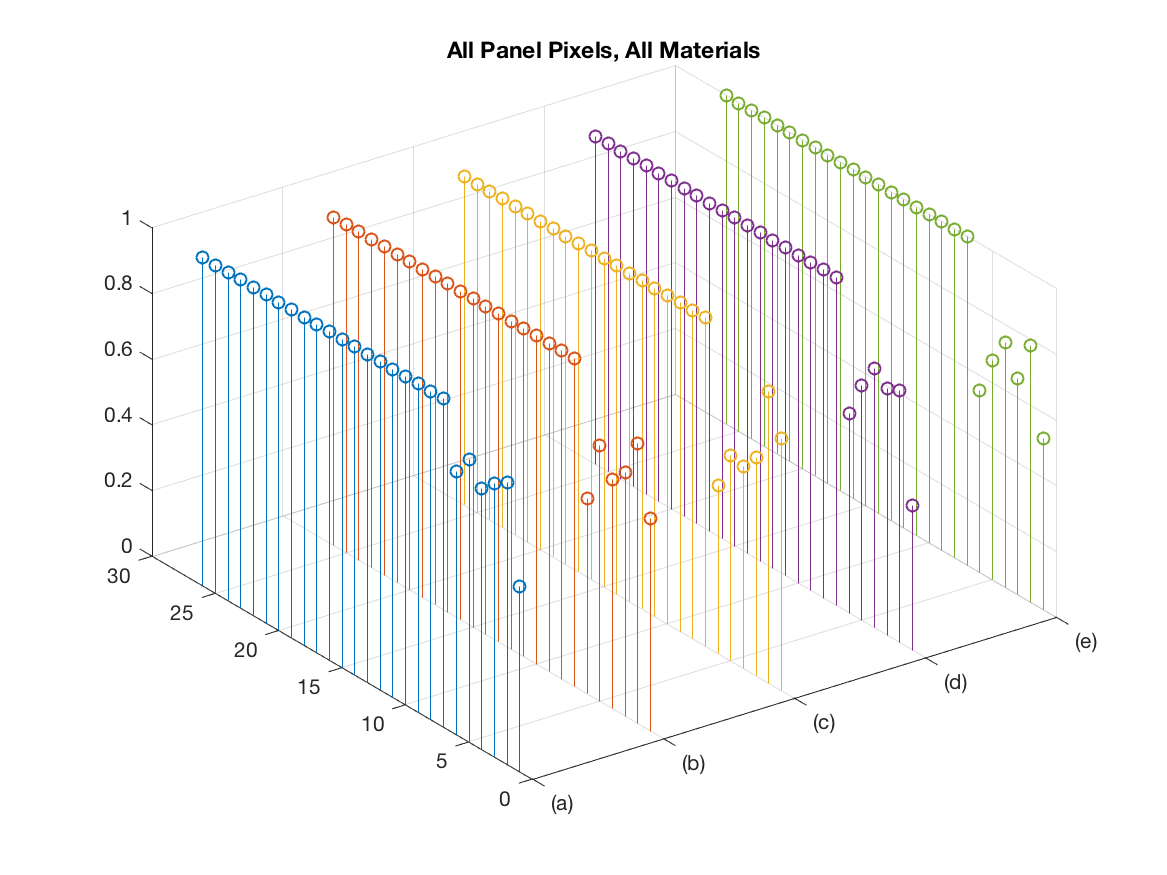
\includegraphics[width=4cm,center]{osp_fcls_ti2_allmaterials}
        \\ All Materials
        \centering
    \end{column}
\end{columns}
\end{frame}

%------------------------------------------------
\begin{frame}{FCLS, OSP Method, TE2 Results}
\begin{columns}
    \begin{column}{0.33\textwidth}
        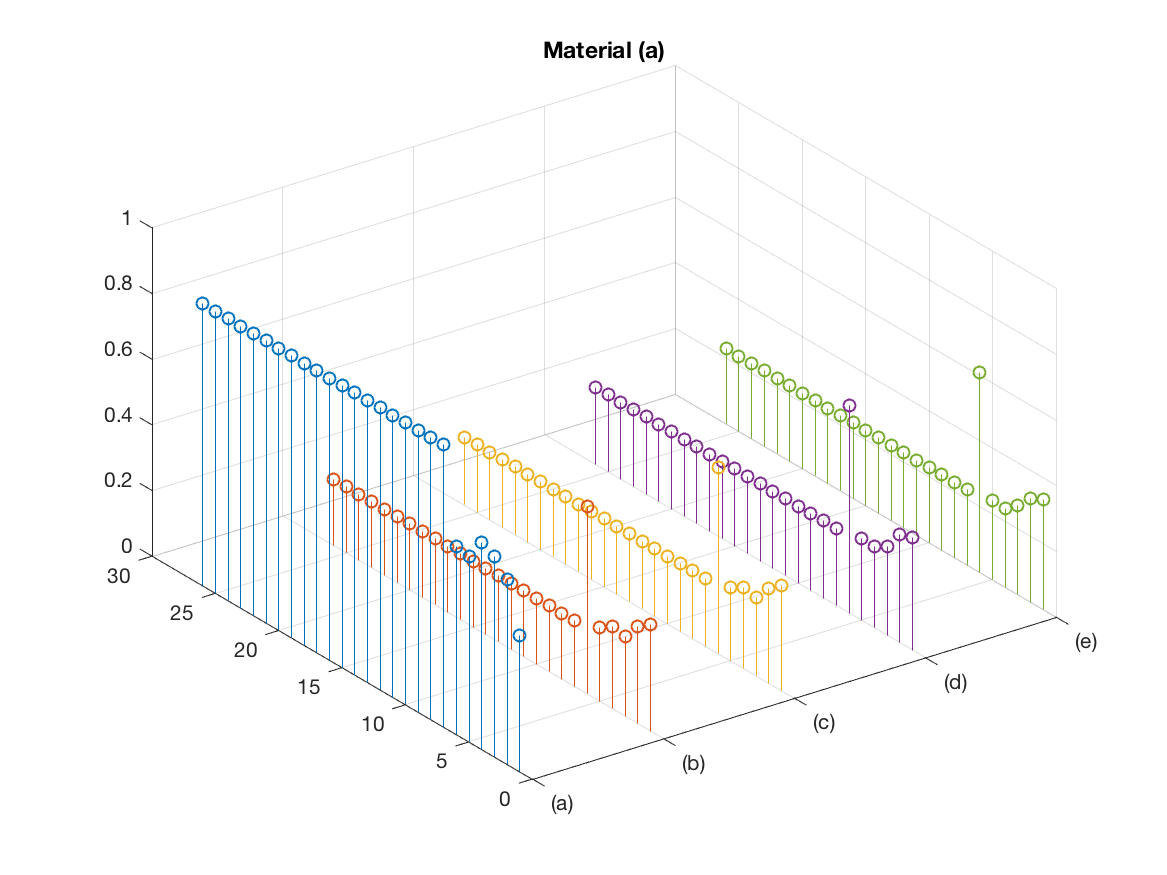
\includegraphics[width=4cm,center]{osp_fcls_te2_material_stem_1}
        \\ Material 1 in all rows
        \centering

        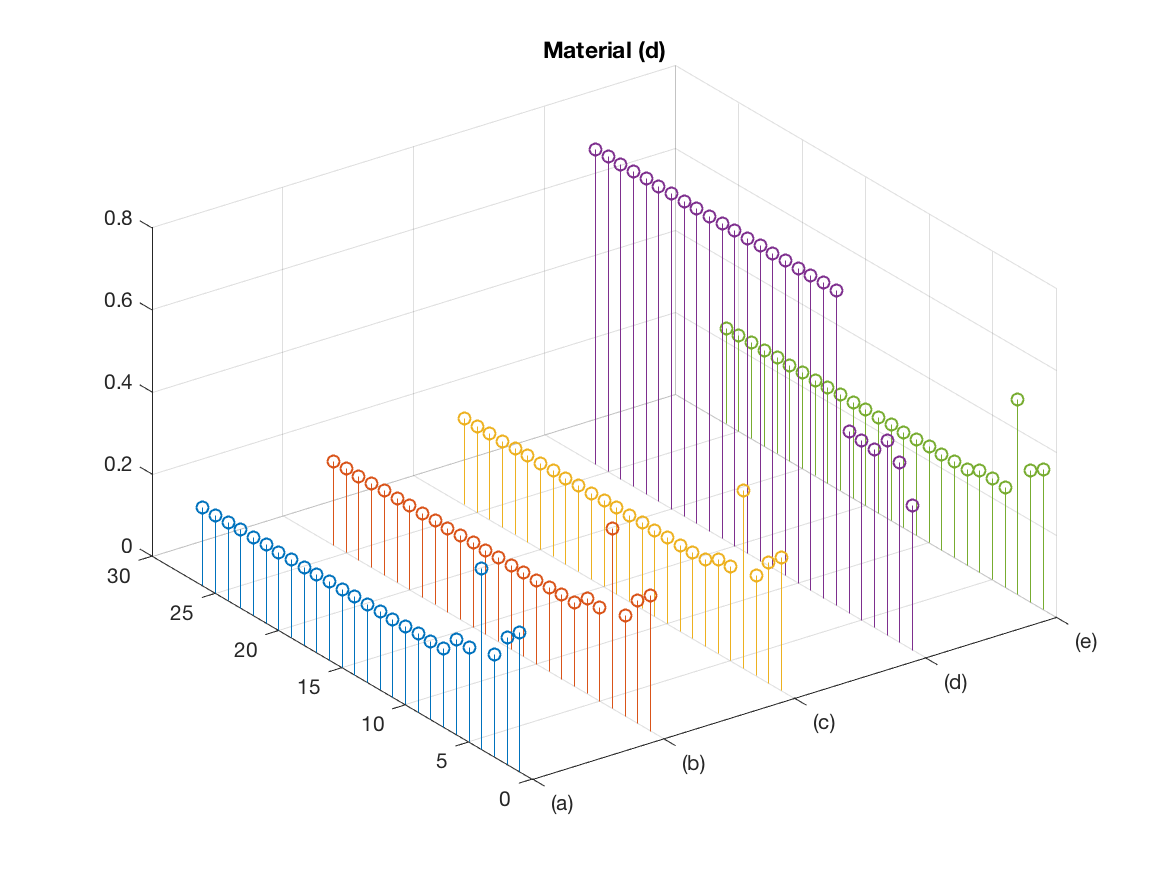
\includegraphics[width=4cm,center]{osp_fcls_te2_material_stem_4}
        \\ Material 4 in all rows
        \centering
    \end{column}
    \begin{column}{0.33\textwidth}
        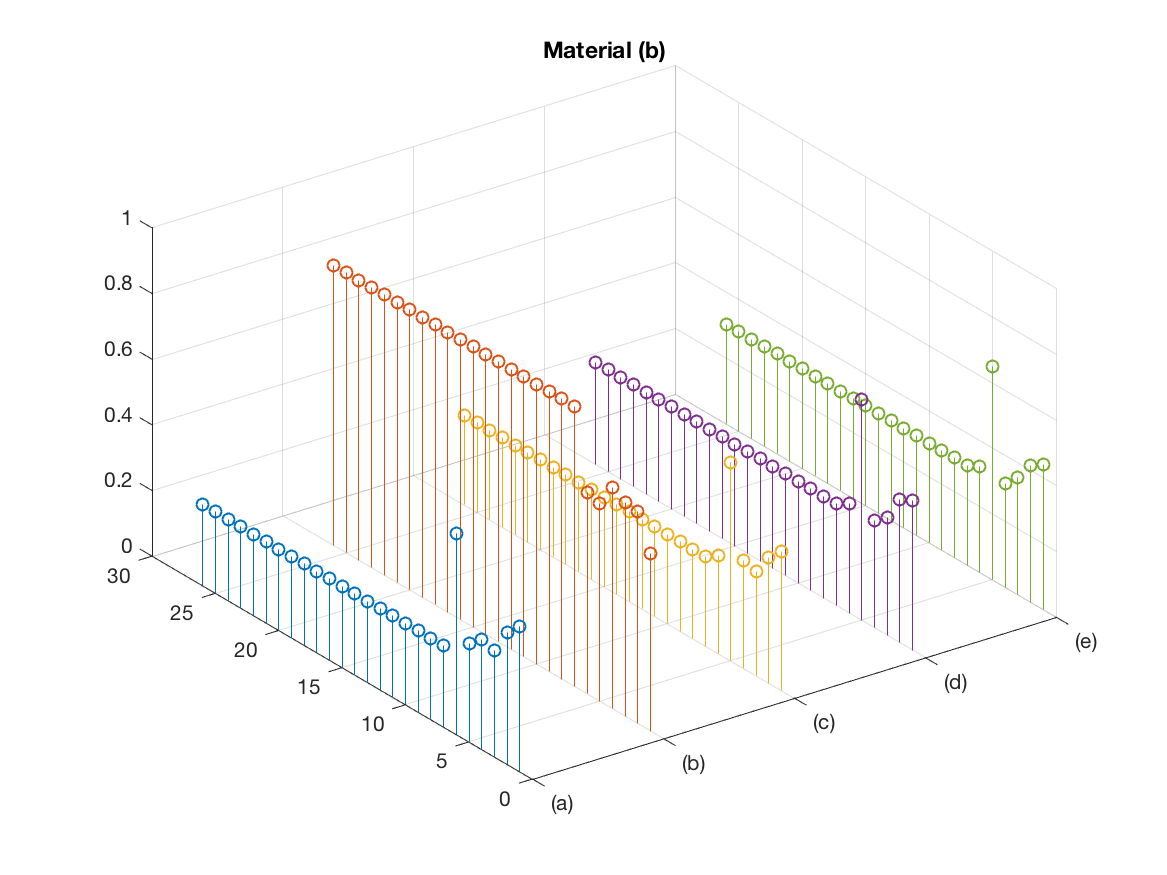
\includegraphics[width=4cm,center]{osp_fcls_te2_material_stem_2}
        \\ Material 2 in all rows
        \centering

        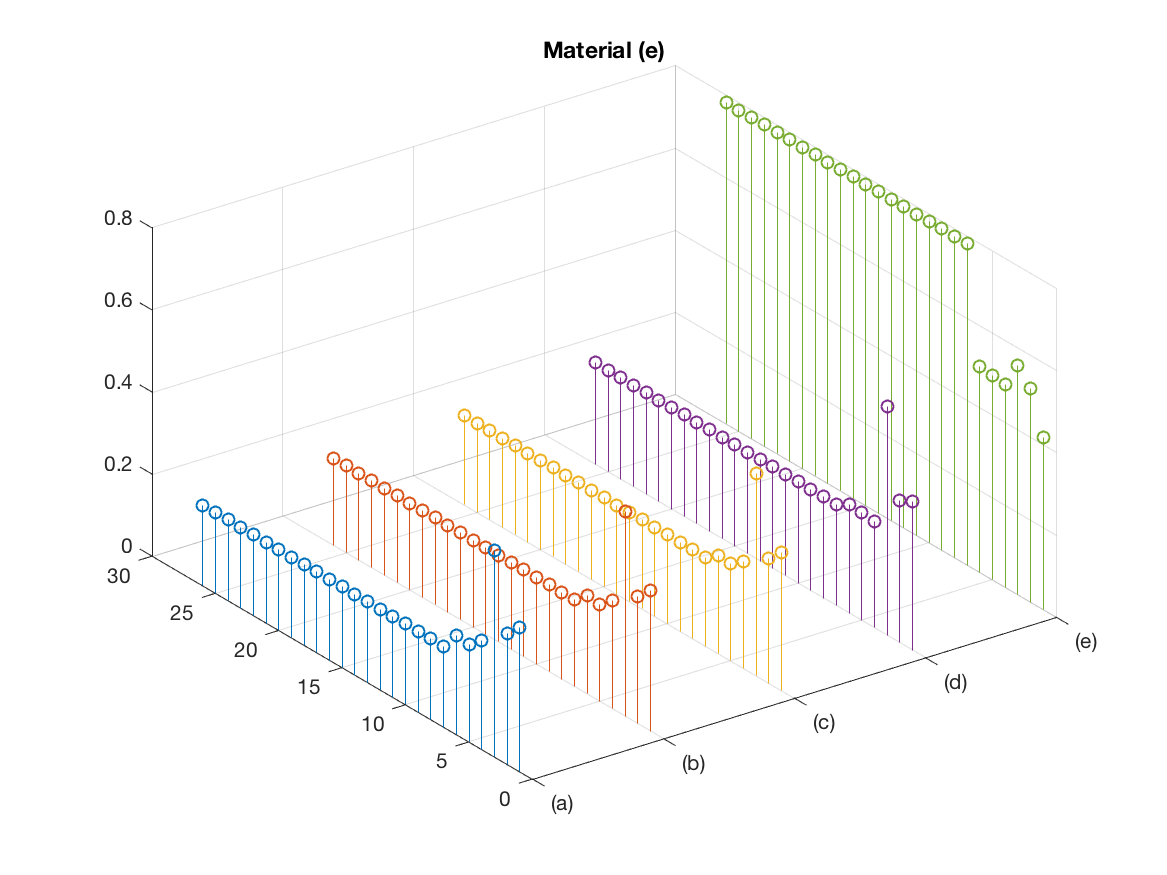
\includegraphics[width=4cm,center]{osp_fcls_te2_material_stem_5}
        \\ Material 5 in all rows
        \centering
    \end{column}
    \begin{column}{0.33\textwidth}
        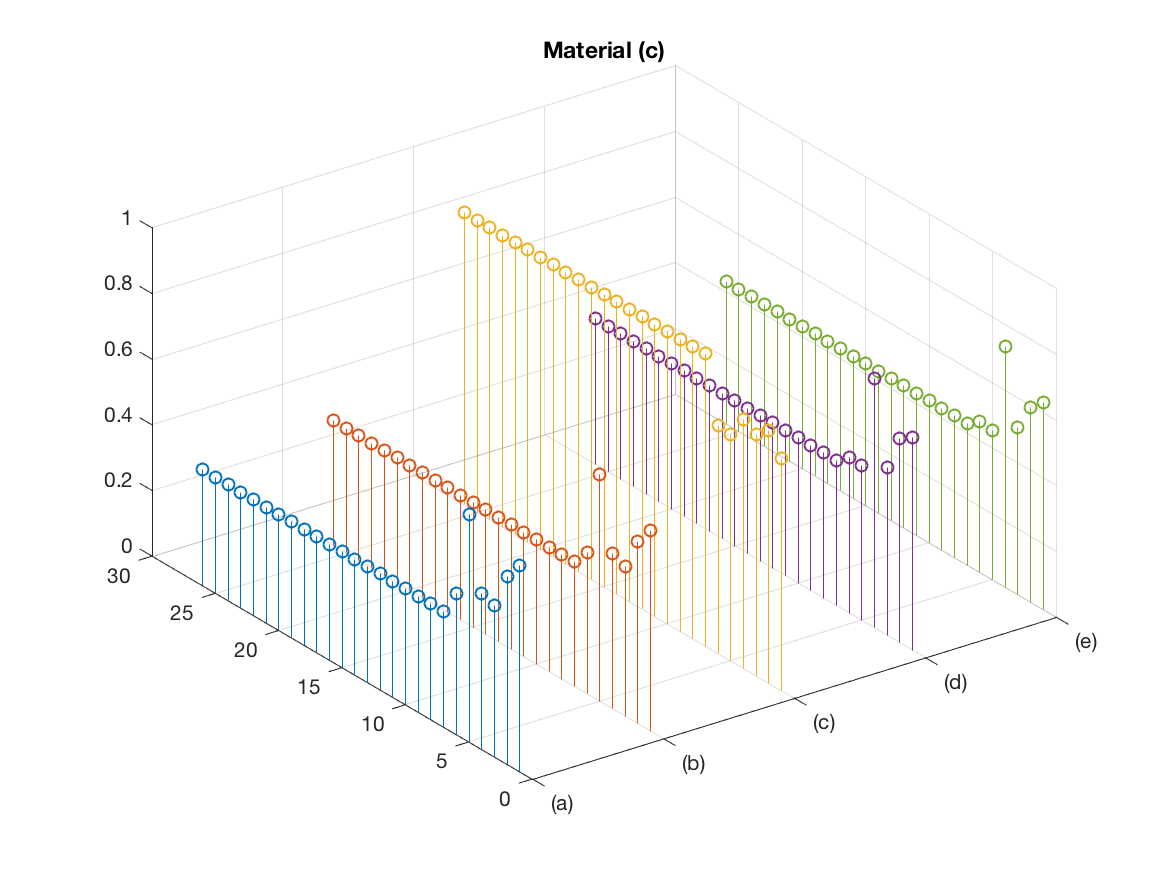
\includegraphics[width=4cm,center]{osp_fcls_te2_material_stem_3}
        \\ Material 3 in all rows
        \centering

        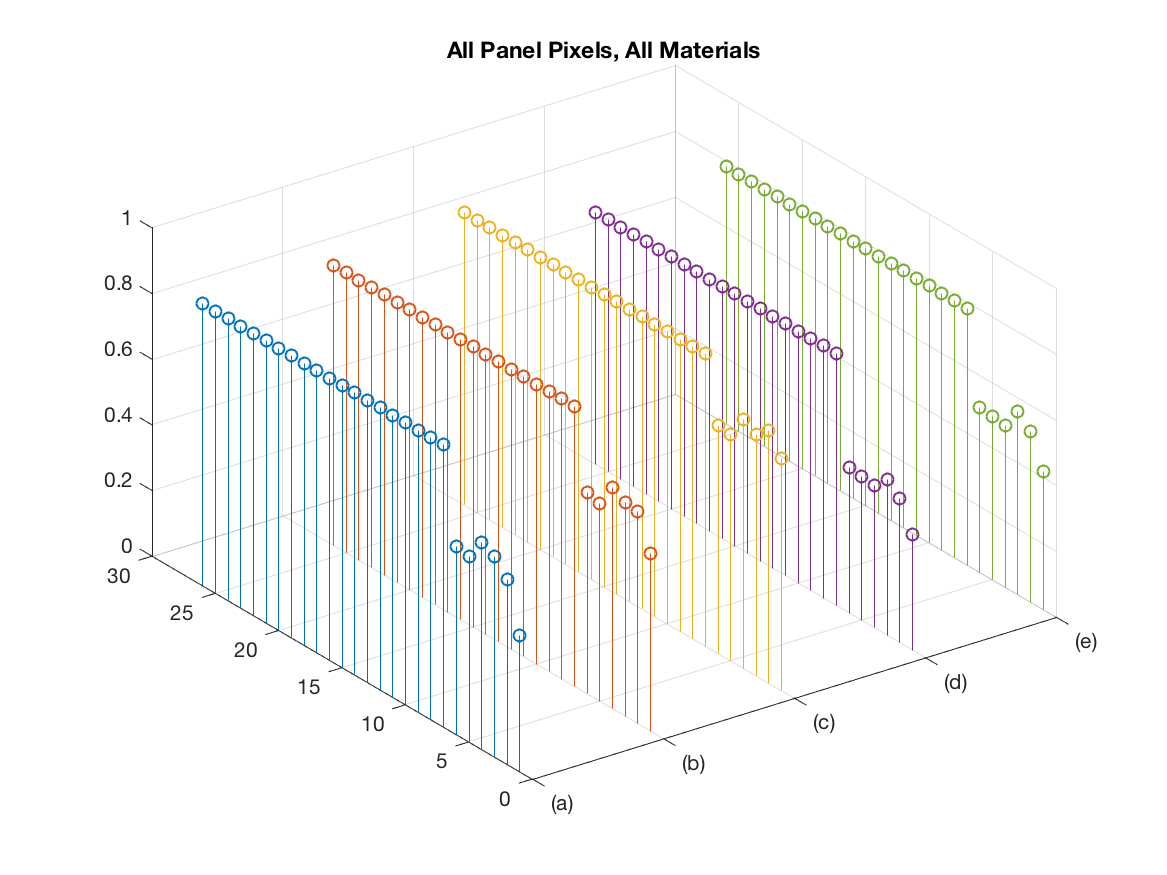
\includegraphics[width=4cm,center]{osp_fcls_te2_allmaterials}
        \\ All Materials
        \centering
    \end{column}
\end{columns}
\end{frame}

%------------------------------------------------
\begin{frame}{Modified FCLS Lagrange Multipler}
\begin{itemize}
\item Initial condition is \(\mathbf{\alpha}^{MFCLS}=\mathbf{\alpha}^{SCLS}\)
\item Compute \(\lambda_1\) and \(\lambda_2\) using constraints \(\sum_{i=1}^{p}\alpha_i = 1\) and \(\sum_{i=1}^{p}|\alpha_i| = 1\)
\item \(\mathbf{\alpha}^{MFCLS}=\mathbf{\alpha}^{SCLS}-\left(\mathbf{M}^T\mathbf{M}\right)^{-1}\left[\lambda_1\mathbf{1}+\lambda_2 sign(\mathbf{\alpha}^{SCLS})\right]\)
\item Iterate if any negative components left
\end{itemize}

\begin{flalign*}
&\begin{bmatrix}
1-\mathbf{1}^T\mathbf{\alpha}^{MFCLS} \\
1-sign(\mathbf{\alpha}_{LS})^T\mathbf{\alpha}^{MFCLS}
\end{bmatrix}
= \\
&\begin{bmatrix}
\mathbf{1}^T(\mathbf{M}^T\mathbf{M})^{-1}\mathbf{1} & \mathbf{1}^T(\mathbf{M}^T\mathbf{M})^{-1} sign(\mathbf{\alpha}_{LS}) \\
sign(\mathbf{\alpha}_{LS})^T(\mathbf{M}^T\mathbf{M})^{-1}\mathbf{1} & sign(\mathbf{\alpha}_{LS}^T) (\mathbf{M}^T\mathbf{M})^{-1} sign(\mathbf{\alpha}_{LS})
\end{bmatrix}
\begin{bmatrix} \lambda_1 \\ \lambda_2 \end{bmatrix} &
\end{flalign*}
\end{frame}

%------------------------------------------------
\begin{frame}{Modified FCLS Lagrange Multipler, TI2 Results}
\begin{columns}
    \begin{column}{0.33\textwidth}
        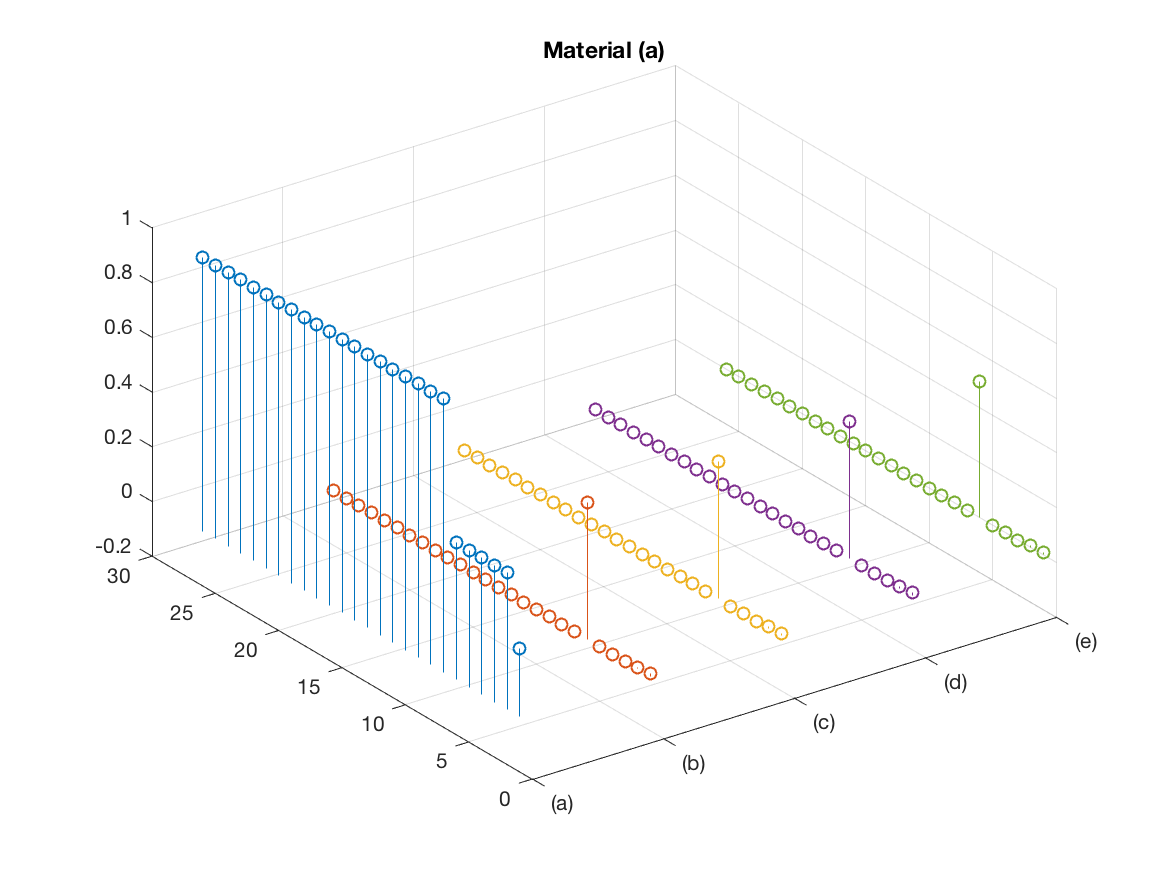
\includegraphics[width=4cm,center]{mfcls2_ti2_material_stem_1}
        \\ Material 1 in all rows
        \centering

        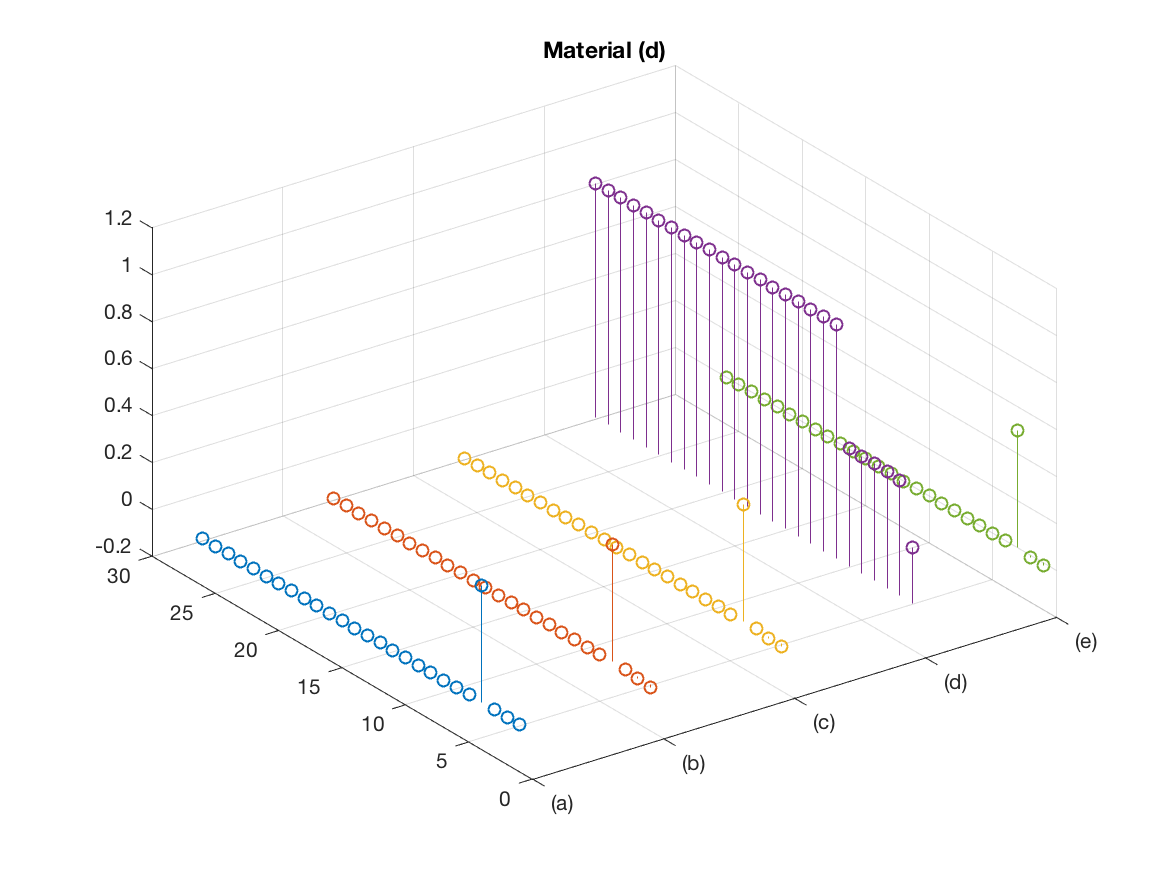
\includegraphics[width=4cm,center]{mfcls2_ti2_material_stem_4}
        \\ Material 4 in all rows
        \centering
    \end{column}
    \begin{column}{0.33\textwidth}
        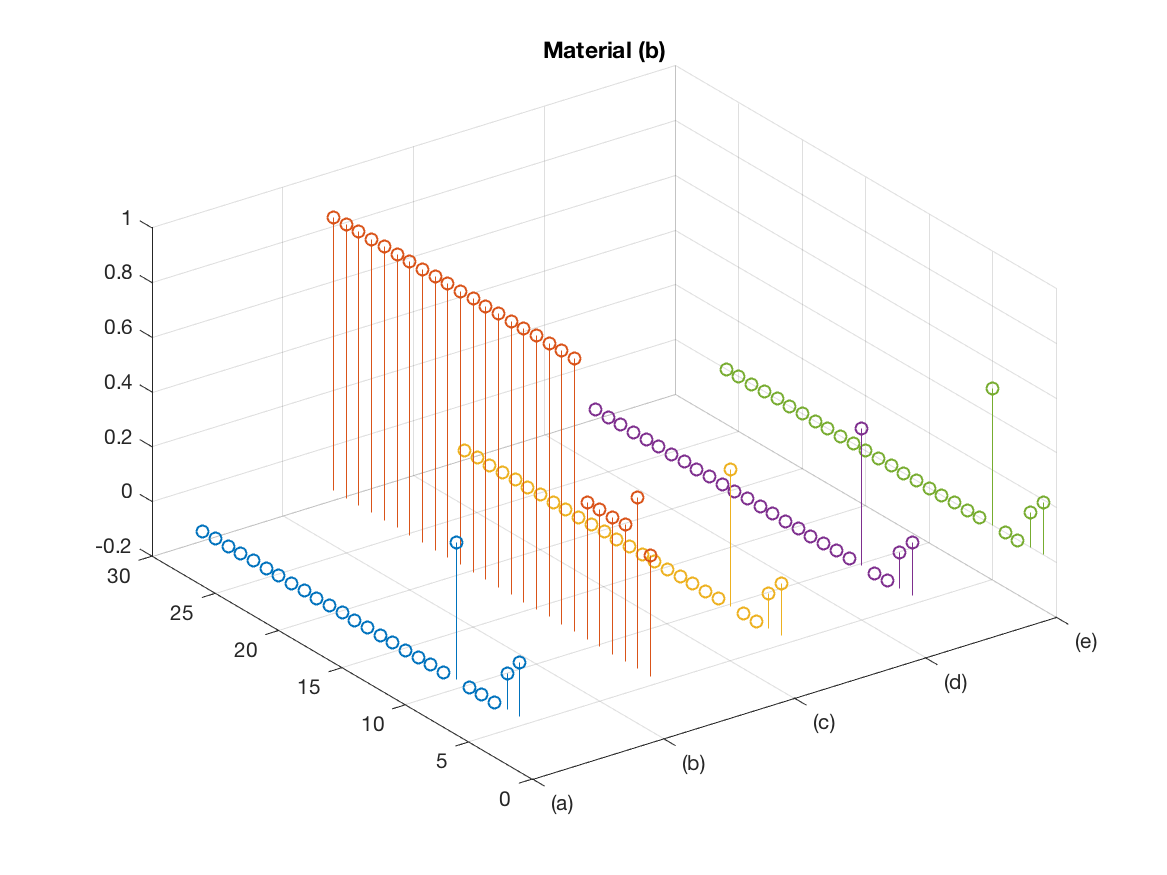
\includegraphics[width=4cm,center]{mfcls2_ti2_material_stem_2}
        \\ Material 2 in all rows
        \centering

        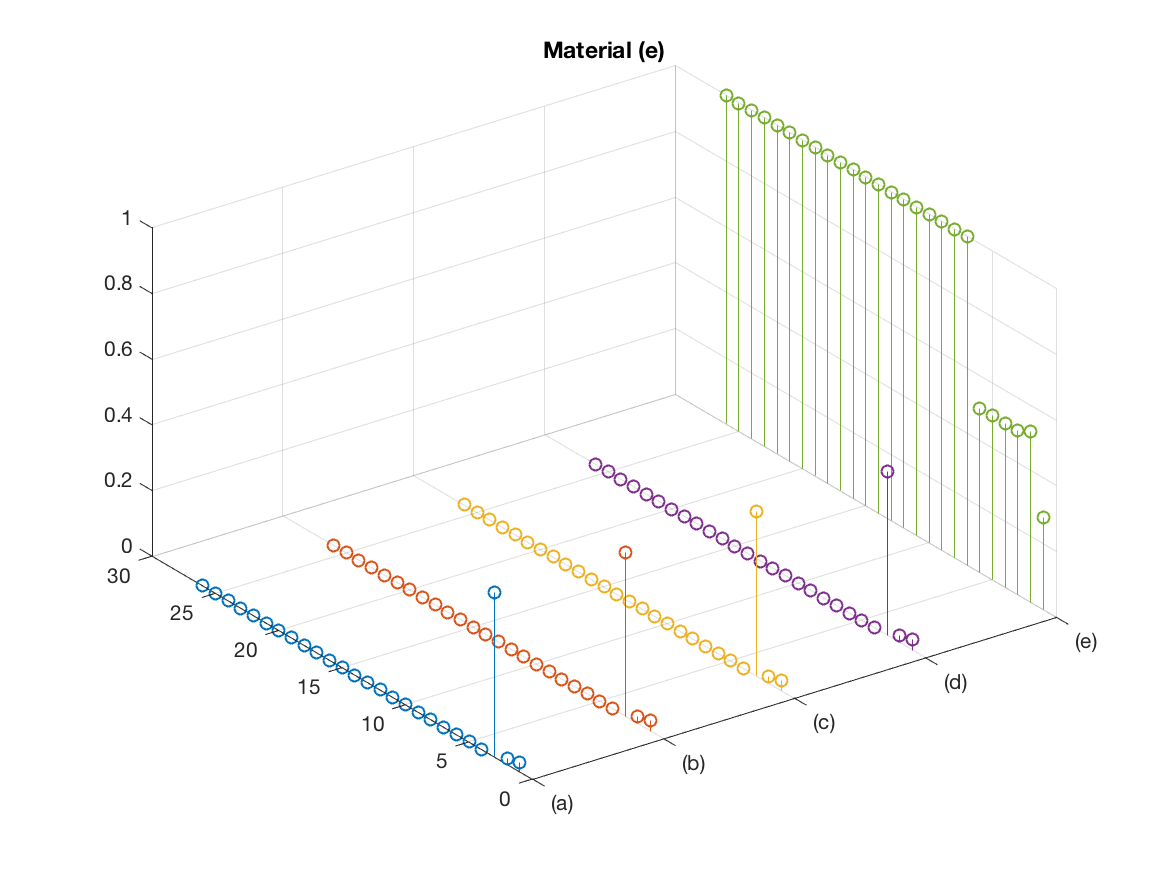
\includegraphics[width=4cm,center]{mfcls2_ti2_material_stem_5}
        \\ Material 5 in all rows
        \centering
    \end{column}
    \begin{column}{0.33\textwidth}
        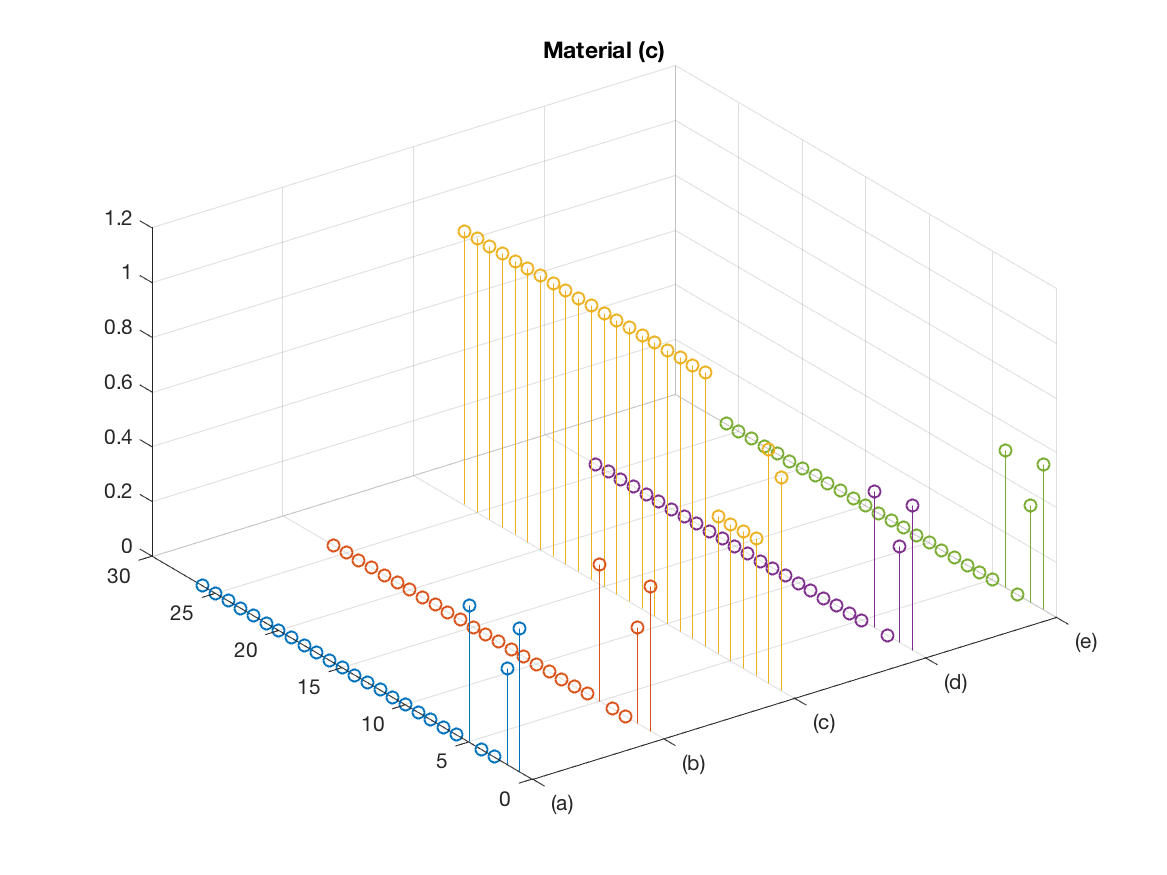
\includegraphics[width=4cm,center]{mfcls2_ti2_material_stem_3}
        \\ Material 3 in all rows
        \centering

        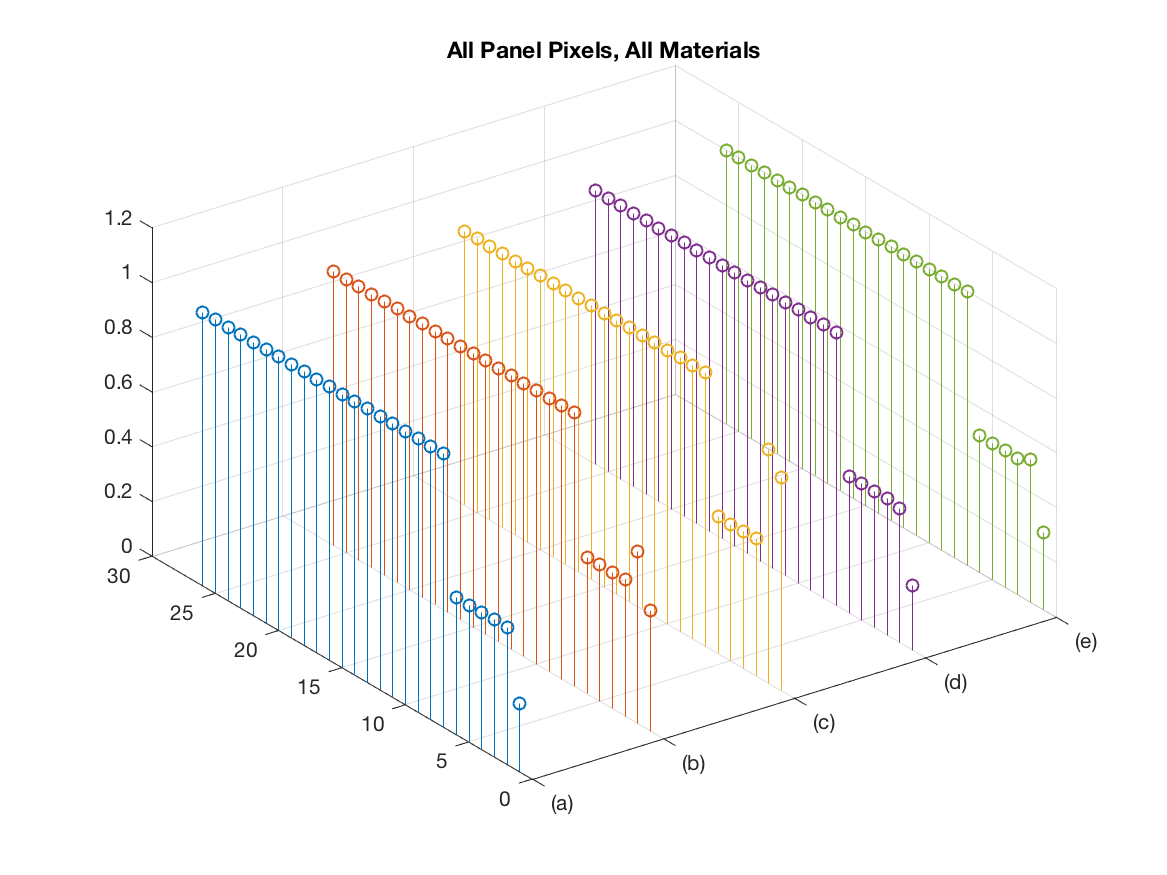
\includegraphics[width=4cm,center]{mfcls2_ti2_allmaterials}
        \\ All Materials
        \centering
    \end{column}
\end{columns}
\end{frame} 

%------------------------------------------------

\begin{frame}{Modified FCLS Lagrange Multipler, TE2 Results}
\begin{columns}
    \begin{column}{0.33\textwidth}
        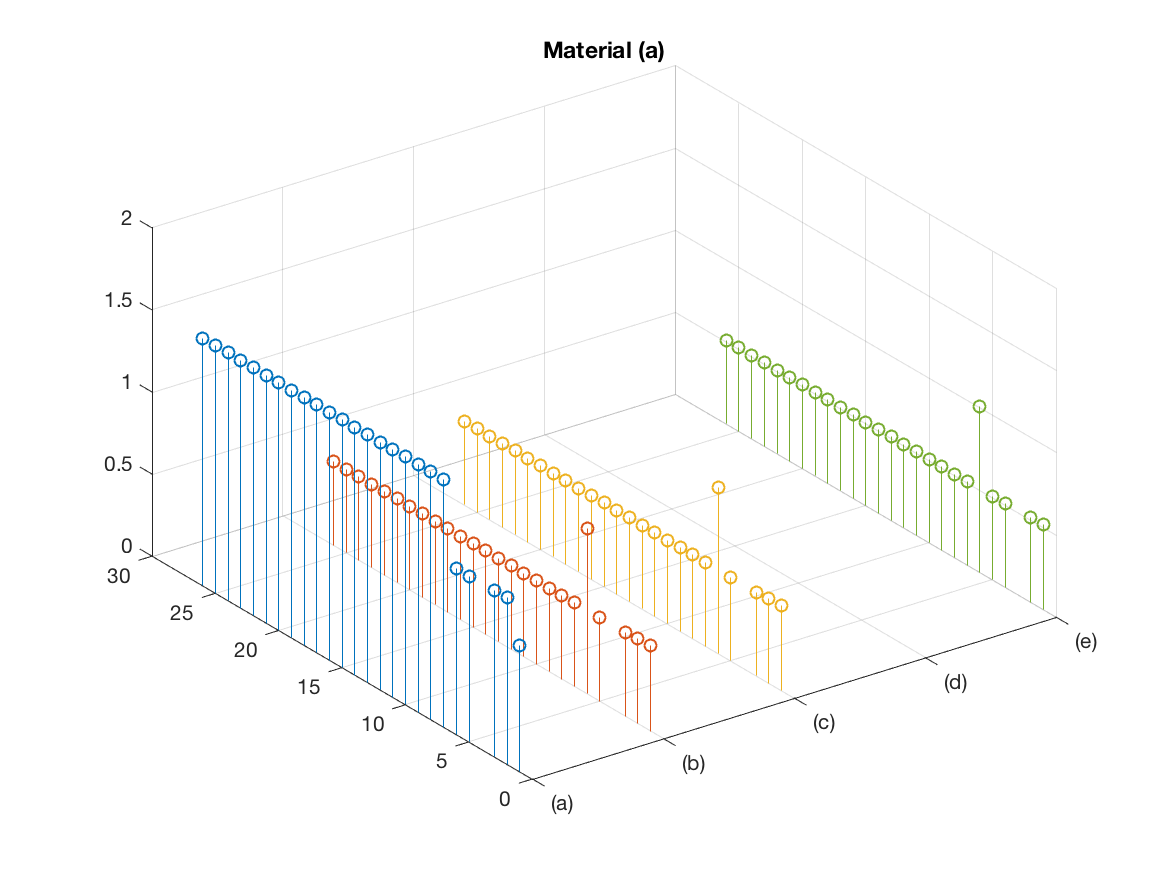
\includegraphics[width=4cm,center]{mfcls2_te2_material_stem_1}
        \\ Material 1 in all rows
        \centering

        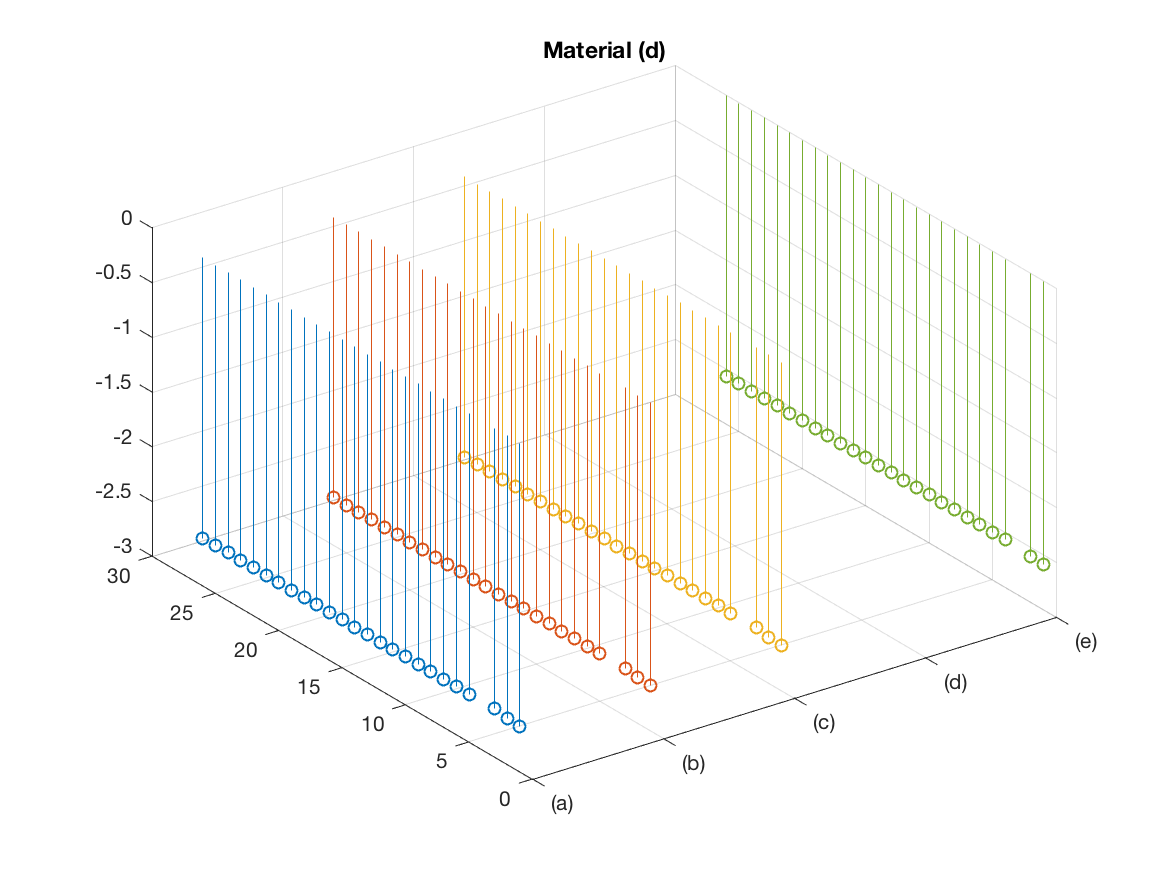
\includegraphics[width=4cm,center]{mfcls2_te2_material_stem_4}
        \\ Material 4 in all rows
        \centering
    \end{column}
    \begin{column}{0.33\textwidth}
        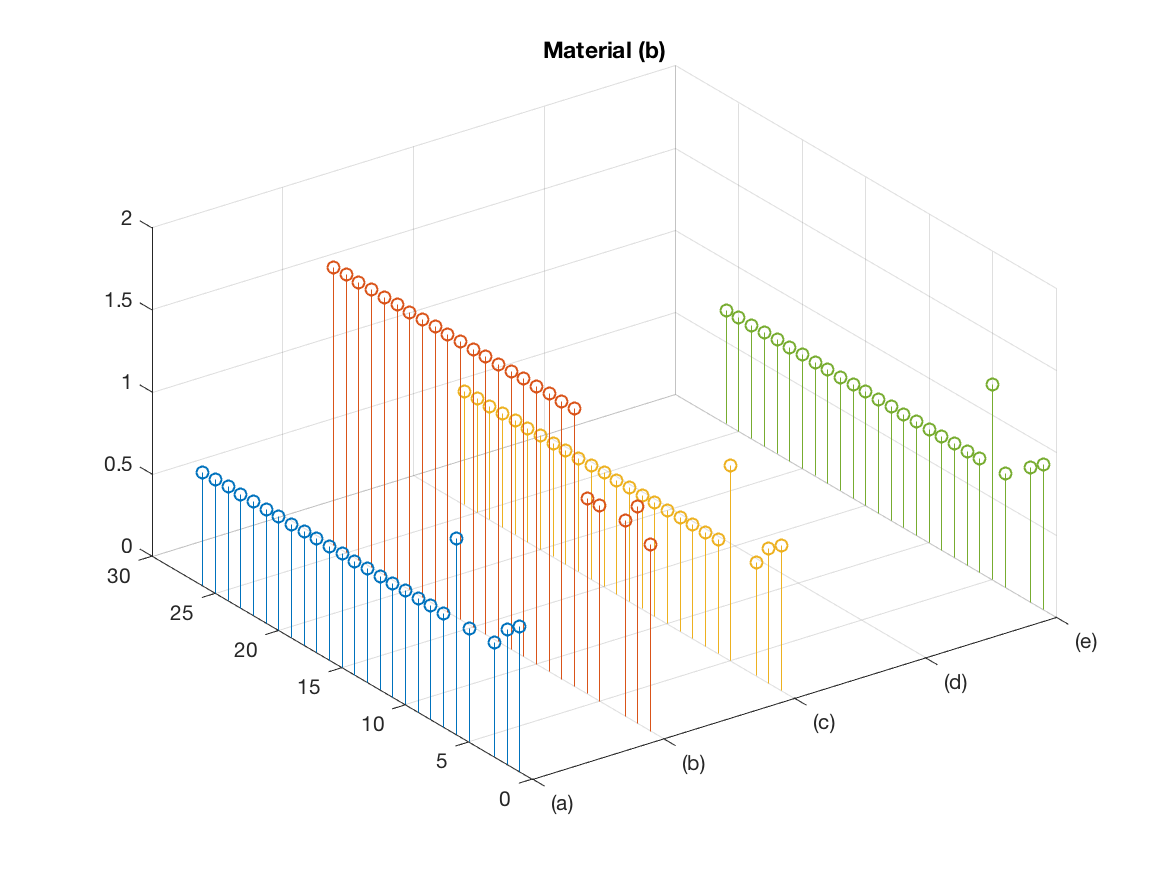
\includegraphics[width=4cm,center]{mfcls2_te2_material_stem_2}
        \\ Material 2 in all rows
        \centering

        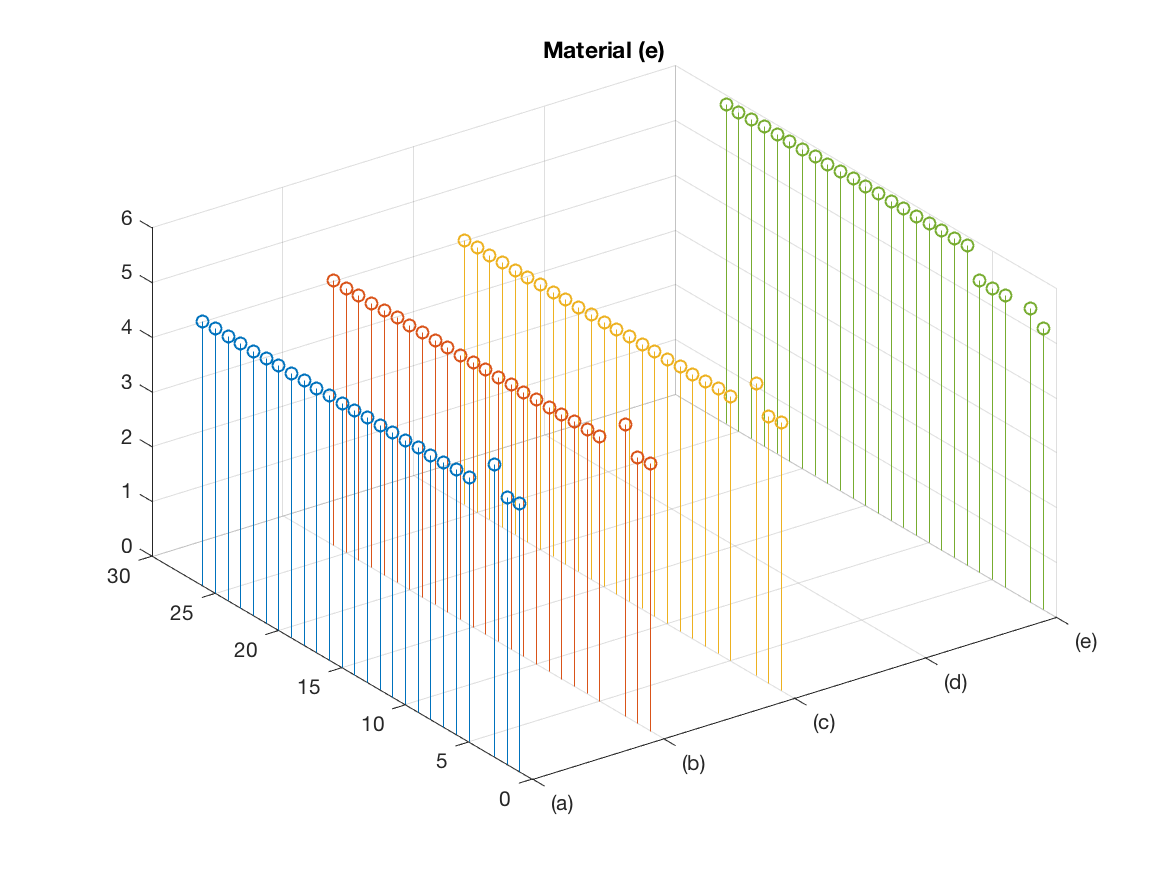
\includegraphics[width=4cm,center]{mfcls2_te2_material_stem_5}
        \\ Material 5 in all rows
        \centering
    \end{column}
    \begin{column}{0.33\textwidth}
        \includegraphics[width=4cm,center]{mfcls2_te2_material_stem_3}
        \\ Material 3 in all rows
        \centering

        \includegraphics[width=4cm,center]{mfcls2_te2_allmaterials}
        \\ All Materials
        \centering
    \end{column}
\end{columns}
\end{frame}

%------------------------------------------------
\begin{frame}{MFCLS Iterative Algorithm}
\begin{itemize}
\item Active set gradient descent method with augmented steering matrix to include ASC and AASC
\item Augments the endmember and pixels to add ASC
\end{itemize}

\begin{align*}
\mathbf{s} = \begin{bmatrix}
\delta\mathbf{r} \\ 1
\end{bmatrix},
\mathbf{N} = \begin{bmatrix}
\delta \mathbf{M} \\ \mathbf{1}^T
\end{bmatrix}
\end{align*}
\end{frame}

%------------------------------------------------
\begin{frame}{Modified FCLS Iterative, TI2 Results}
\begin{columns}
    \begin{column}{0.33\textwidth}
        \includegraphics[width=4cm,center]{mfcls_ti2_material_stem_1}
        \\ Material 1 in all rows
        \centering

        \includegraphics[width=4cm,center]{mfcls_ti2_material_stem_4}
        \\ Material 4 in all rows
        \centering
    \end{column}
    \begin{column}{0.33\textwidth}
        \includegraphics[width=4cm,center]{mfcls_ti2_material_stem_2}
        \\ Material 2 in all rows
        \centering

        \includegraphics[width=4cm,center]{mfcls_ti2_material_stem_5}
        \\ Material 5 in all rows
        \centering
    \end{column}
    \begin{column}{0.33\textwidth}
        \includegraphics[width=4cm,center]{mfcls_ti2_material_stem_3}
        \\ Material 3 in all rows
        \centering

        \includegraphics[width=4cm,center]{mfcls_ti2_allmaterials}
        \\ All Materials
        \centering
    \end{column}
\end{columns}
\end{frame}

%------------------------------------------------
\begin{frame}{Modified FCLS Iterative, TE2 Results}
\begin{columns}
    \begin{column}{0.33\textwidth}
        \includegraphics[width=4cm,center]{mfcls_te2_material_stem_1}
        \\ Material 1 in all rows
        \centering

        \includegraphics[width=4cm,center]{mfcls_te2_material_stem_4}
        \\ Material 4 in all rows
        \centering
    \end{column}
    \begin{column}{0.33\textwidth}
        \includegraphics[width=4cm,center]{mfcls_te2_material_stem_2}
        \\ Material 2 in all rows
        \centering

        \includegraphics[width=4cm,center]{mfcls_te2_material_stem_5}
        \\ Material 5 in all rows
        \centering
    \end{column}
    \begin{column}{0.33\textwidth}
        \includegraphics[width=4cm,center]{mfcls_te2_material_stem_3}
        \\ Material 3 in all rows
        \centering

        \includegraphics[width=4cm,center]{mfcls_te2_allmaterials}
        \\ All Materials
        \centering
    \end{column}
\end{columns}
\end{frame}

%------------------------------------------------
\begin{frame}{Numerical Results, Accuracy and Timing}
\begin{table}[!h]
    \caption{I. Algorithm accuracy in MSE}
    \centering
    \begin{tabular}{|c|c|c|c|c|c|}
    \hline
        & Active Set & Geometric & OSP & MFCLS 1 & MFCLS 2 \\ \hline
    TI2 & 0.003489& 0.00394& 0.01672& 0.003536& 0.003538\\ \hline
    TE2 & 0.709771& 0.13506& 0.02976& 5.677302& 143345.3 \\ \hline
    \end{tabular}
\end{table}

\begin{table}[!h]
    \caption{II. Algorithm timing in seconds}
    \centering
    \begin{tabular}{|c|c|c|c|c|c|}
    \hline
     Active Set & Geometric & OSP & MFCLS 1 & MFCLS 2 \\ \hline
    3.263822& 1.762295& 1.880125&  2.453860& 9.055446 \\ \hline
    \end{tabular}
\end{table}
\end{frame}

%------------------------------------------------
\begin{frame}{Direct MNF}
    \begin{itemize}
        \item Try and use MNF for FCLS
        \item Tried using augmented endmember matrix and pixels for ASC
        \item Also tried directly normalizing abundance on each iteration
        \item Tried both alternating least squares and multiplicative update
        \item Initialize the \(\mathbf{W}\) matrix to \(\mathbf{M}\)
    \end{itemize}

\begin{align*}
\mathbf{s} = \begin{bmatrix}
\delta\mathbf{r} \\ 1
\end{bmatrix},
\mathbf{N} = \begin{bmatrix}
\delta \mathbf{M} \\ \mathbf{1}^T
\end{bmatrix}
\end{align*}

\end{frame}

%------------------------------------------------
\begin{frame}{TI2 Direct NMF}
\begin{columns}
    \begin{column}{0.33\textwidth}
        \includegraphics[width=4cm,center]{reflectance}
        \\ Ground Truth Endmembers
        \centering
    \end{column}
    \begin{column}{0.33\textwidth}
        \includegraphics[width=4cm,center]{other_ti2_nmf_endmembers.png}
        \\ NMF Computed Endmembers
        \centering
    \end{column}
    \begin{column}{0.33\textwidth}
        \includegraphics[width=4cm,center]{other_ti2_nmf_allmaterials.png}
        \\ NMF Computed Abundance
        \centering
    \end{column}
\end{columns}
\end{frame}

%------------------------------------------------
\begin{frame}{TE2 Direct NMF}
\begin{columns}
    \begin{column}{0.33\textwidth}
        \includegraphics[width=4cm,center]{reflectance}
        \\ Ground Truth Endmembers
        \centering
    \end{column}
    \begin{column}{0.33\textwidth}
        \includegraphics[width=4cm,center]{other_te2_nmf_endmembers.png}
        \\ NMF Computed Endmembers
        \centering
    \end{column}
    \begin{column}{0.33\textwidth}
        \includegraphics[width=4cm,center]{other_te2_nmf_allmaterials.png}
        \\ NMF Computed Abundance
        \centering
    \end{column}
\end{columns}
\end{frame}

%------------------------------------------------
\begin{frame}{NMF Hoyer Sparsity Algorithm}
    \begin{columns}
        \begin{column}{1\textwidth}
            \includegraphics[width=10cm,left]{hoyer.png}
        \end{column}
    \end{columns}
\end{frame}

%------------------------------------------------
\begin{frame}{NMF Hoyer Sparsity Algorithm}
    \includegraphics[width=10cm,center]{NMF}
\end{frame}

%------------------------------------------------
\begin{frame}{TI2 NMF with Hoyer Sparsity = 0.7, Normalized ASC}
\begin{columns}
    \begin{column}{0.33\textwidth}
        \includegraphics[width=4cm,center]{reflectance}
        \\ Ground Truth Endmembers
        \centering
    \end{column}
    \begin{column}{0.33\textwidth}
        \includegraphics[width=4cm,center]{nmf_endmembers_ti2_70.png}
        \\ NMF Computed Endmembers
        \centering
    \end{column}
    \begin{column}{0.33\textwidth}
        \includegraphics[width=4cm,center]{nmf_abundance_ti2_70_allmaterials.png}
        \\ NMF Computed Abundance
        \centering
    \end{column}
\end{columns}
\end{frame}

%------------------------------------------------
\begin{frame}{TE2 NMF with Hoyer Sparsity = 0.7, Normalized  ASC}
\begin{columns}
    \begin{column}{0.33\textwidth}
        \includegraphics[width=4cm,center]{reflectance}
        \\ Ground Truth Endmembers
        \centering
    \end{column}
    \begin{column}{0.33\textwidth}
        \includegraphics[width=4cm,center]{nmf_endmembers_te2_70.png}
        \\ NMF Computed Endmembers
        \centering
    \end{column}
    \begin{column}{0.33\textwidth}
        \includegraphics[width=4cm,center]{nmf_abundance_te2_70_allmaterials.png}
        \\ NMF Computed Abundance
        \centering
    \end{column}
\end{columns}
\end{frame}

%------------------------------------------------
\begin{frame}{TI2 NMF with Hoyer Sparsity = 0.95, Normalized  ASC}
\begin{columns}
    \begin{column}{0.33\textwidth}
        \includegraphics[width=4cm,center]{reflectance}
        \\ Ground Truth Endmembers
        \centering
    \end{column}
    \begin{column}{0.33\textwidth}
        \includegraphics[width=4cm,center]{nmf_endmembers_ti2_95.png}
        \\ NMF Computed Endmembers
        \centering
    \end{column}
    \begin{column}{0.33\textwidth}
        \includegraphics[width=4cm,center]{nmf_abundance_ti2_95_allmaterials.png}
        \\ NMF Computed Abundance
        \centering
    \end{column}
\end{columns}
\end{frame}

%------------------------------------------------
\begin{frame}{TE2 NMF with Hoyer Sparsity = 0.95, Normalized  ASC}
\begin{columns}
    \begin{column}{0.33\textwidth}
        \includegraphics[width=4cm,center]{reflectance}
        \\ Ground Truth Endmembers
        \centering
    \end{column}
    \begin{column}{0.33\textwidth}
        \includegraphics[width=4cm,center]{nmf_endmembers_te2_95.png}
        \\ NMF Computed Endmembers
        \centering
    \end{column}
    \begin{column}{0.33\textwidth}
        \includegraphics[width=4cm,center]{nmf_abundance_te2_95_allmaterials.png}
        \\ NMF Computed Abundance
        \centering
    \end{column}
\end{columns}
\end{frame}

%------------------------------------------------
\begin{frame}{Minimum Volume Constrained NMF}
\begin{itemize}
\item Minimize the LSE subject to ANC and ASC and minimum volume
\item Algorithm in paper uses gradient descent of objective function and PCA projection to measure volume
\item At each iteration impose the ASC via abundance matrix augmentation
\end{itemize}

\begin{align*}
    & min\{f(\mathbf{M}, \mathbf{A}) = 1/2\| \mathbf{R} - \mathbf{M}\mathbf{A} \|_F^2 + \lambda Vol(\mathbf{M})\} \\
    & \mathbf{M} \succeq 0, \mathbf{A} \succeq 0, \mathbf{1}^T\mathbf{A} = \mathbf{1}
\end{align*}
\end{frame}

\begin{frame}{Minimum Volume Constrained NMF}
\includegraphics[width=10cm, center]{mvc_mnf}
\end{frame}

%------------------------------------------------
\begin{frame}{Conclusions}

\begin{itemize}
\item FCLS and MFCLS works well with TI2
    \begin{itemize}
        \item TI2 pixels are in the range space of the endmembers
    \end{itemize}
\item FCLS and MFCLS does not work well for TE2
    \begin{itemize}
        \item TE2 pixels are not in the range space of the endmembers because of the background
    \end{itemize}
\item NMF can be used to do linear unmixing of HSI data into constituent materials
    \begin{itemize}
        \item Other constraints are necessary to produce good results
    \end{itemize}
\end{itemize}

\end{frame}

%------------------------------------------------
\begin{frame}
\frametitle{References}
\footnotesize{
\begin{thebibliography}{99}

\bibitem[chang_2013]{p1} Chein-I Chang (2013)
\newblock Hyperspectral Data Processing: Algorithms Design and Analysis
\newblock \emph{Wiley}, Appendix A.4.2

\bibitem[Heinz_chang]{p1} Daniel Heinz, and Chein-I Chang (2001)
\newblock Fully Constrained Least Squares Linear Spectral Mixture Analysis Method for Material Quantification in Hyperspectral Imagery
\newblock \emph{IEEE Transactions on Geoscience and Remote Sensing, Vol. 39, No. 3}

\bibitem[Lee_2001]{p1} Daniel D. Lee, and H. Sebastian Seung
\newblock Algorithms for Non-negative Matrix Factorization
\newblock \emph{Advances in Neural Information Processing Systems} 556 -- 562.

\bibitem[Lee_1999]{p1} Daniel D. Lee, and H. Sebastian Seung (October 1999)
\newblock Learning the parts of objects by non-negative matrix factorization
\newblock \emph{Nature} 401, 788 -- 791.

\end{thebibliography}
}
\end{frame}

%------------------------------------------------
\begin{frame}
\frametitle{References}
\footnotesize{
\begin{thebibliography}{99}

\bibitem[Wong_chang]{p1} Englin Wong, and Chein-I Chang (2012)
\newblock Modified fully abundance-constrained spectral unmixing
\newblock \emph{Proc. SPIE 8539, High-Performance Computing in Remote Sensing II}

\bibitem[Lidan_miao]{p1} Lidan Miao, Hairong Qi (2007)
\newblock Endmember Extraction From Highly Mixed Data Using Minimum Volume Constrained Nonnegative Matrix Factorization
\newblock \emph{IEEE Transactions on Geoscience and Remote Sensing, Vol. 45, No. 3}

\bibitem[Liguo_Wang]{p1} Liguo Wang, and Danfeng Liu, and Qunming Wang (June 2013)
\newblock Geometric Method of Fully Constrained Least Squares Linear Spectral Mixture Analysis
\newblock \emph{IEEE Transactions on Geoscience and Remote Sensing, Vol. 51, No. 6}

\bibitem[Mandula]{p1} Ondrej Mandula (2011)
\newblock \emph{https://github.com/aludnam/MATLAB/tree/master/nmfpack}

\end{thebibliography}
}
\end{frame}

%------------------------------------------------
\begin{frame}
\frametitle{References}
\footnotesize{
\begin{thebibliography}{99}

\bibitem[Hoyer_2002]{p1} Patrik Hoyer (February 2002)
\newblock Non-negative Sparse Coding
\newblock \emph{Neural Networks for Signal Processing} 12, 557 -- 565.

\bibitem[Hoyer_2004]{p1} Patrik Hoyer (November 2004)
\newblock Non-negative Matrix Factorization with Sparseness Constraints
\newblock \emph{Machine Learning Research} 5, 1457 -- 1469.

\bibitem[Sen_Jia]{p1} Sen Jia, and Yuntao Qian (January 2009)
\newblock Constrained Nonnegative Matrix Factorization for Hyperspectral Unmixing
\newblock \emph{IEEE Transactions on Geoscience and Remote Sensing, Vol. 47, No. 1}

\end{thebibliography}
}
\end{frame}

%------------------------------------------------

\end{document} 
